
%%%%%%%%%%%%%%%%
%%% Figure 1 %%%
%%%%%%%%%%%%%%%%
%\begin{figure}[h]
%\begin{center}
%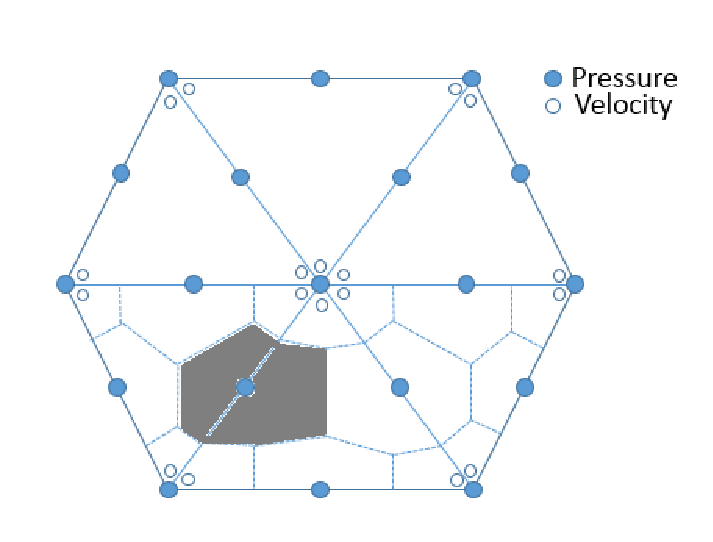
\includegraphics[width=.5\textwidth]{./Pics/P1DGP2.pdf}
%\caption{2D representation of the $P_{1}DGP_{2}$ element pairs used in this work. Shaded areas denote control volumes (in which saturation field is stored), blue points represent the pressure nodes and white points the velocity nodes.}
%\label{fig:fem_cv}
%\end{center}
%\end{figure}
%\clearpage

%%%%%%%%%%%%%%%%
%%% Figure 2 %%%
%%%%%%%%%%%%%%%%
%\begin{figure}[h] 
%\begin{center}
%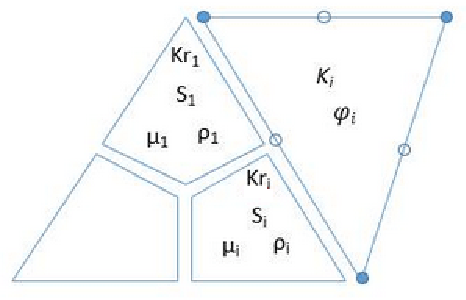
\includegraphics[width=.5\textwidth]{./Pics/element_n.pdf}
%\caption{Porosity $\phi_{i}$, and permeability $K_{i}$ are associated to the elements. The velocity and pressure are associated to the element corners and the mid-points as described in fig.\ref{fig:fem_cv}; three CVs fit into a $2$D element. Saturation and saturation-dependent variables are stored CV-wise.}
%\label{fig:fem_elem}
%\end{center}
%\end{figure}
%\clearpage

%%%%
%%%%  FIGURE 
%%%%
\begin{figure}[h]
\centering
\vbox{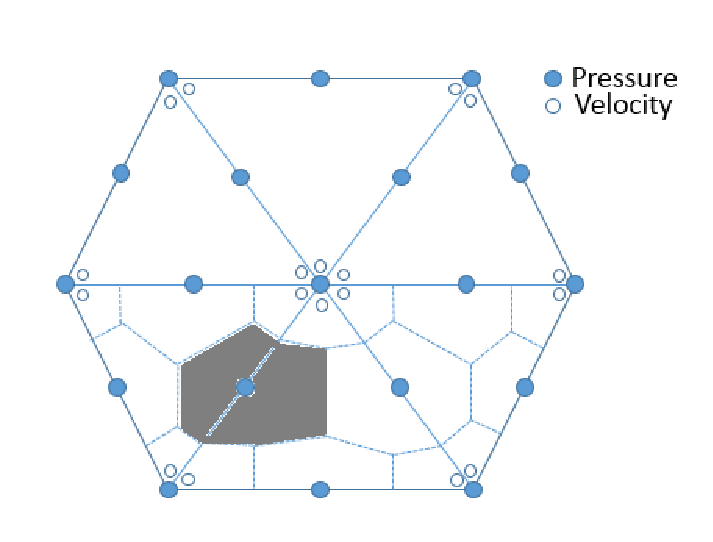
\includegraphics[width=.5\textwidth]{./Pics/P1DGP2.pdf}}
\caption{2D representation of \PN[1]{2} element pairs used in this work. Shaded areas denote control volumes across two contiguous elements. Blue and white circles represent pressure and velocity nodes, respectively.}
\label{fig:fem_cv}
\end{figure}

\clearpage

%%%%
%%%%  FIGURE
%%%%
\begin{figure}[h]
\centering
\vbox{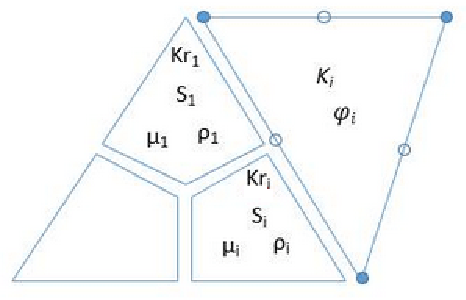
\includegraphics[width=.5\textwidth]{./Pics/element_n.pdf}}
\caption{This is a graphical representation of two different element types. Element A is the \PN[1]{2}, while element B is the \PN[1]{1}. Porosity $\phi_{i}$ and permeability $K_{i}$ are CV-wise quantities, whereas velocity and pressure are primarily represented in FE space. Scalar fields (such saturation, density, viscosity etc) are also represented in CV space.}
}
\label{fig:fem_elem}
\end{figure}

\clearpage

%%%%
%%%%  FIGURE 1
%%%%
\begin{figure}[h]
\centering
\vbox{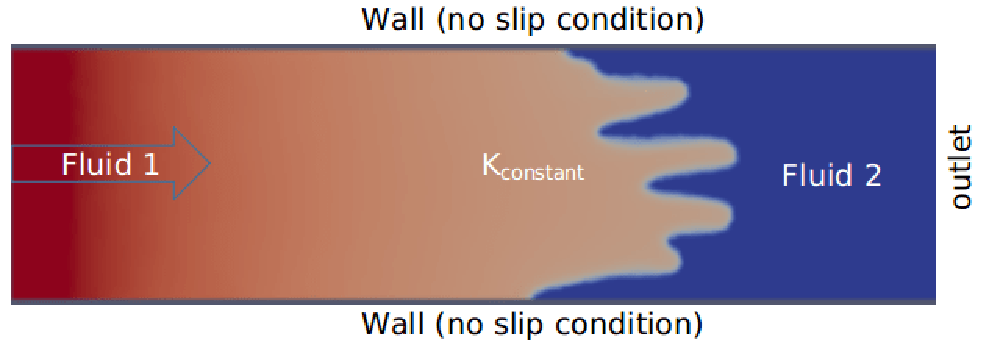
\includegraphics[width=0.75\textwidth]{./Pics/phase_vol_frac_uni_perm_1.pdf}}
\caption{Schematics of formation of flow instabilities during injection of a pure low viscosity fluid (red) into a domain saturated with a second fluid (dark blue). The ratio of viscosity between the two fluids is 5. In this case, the initially piston shape front collapses leading to the formation of several fingers.}
\label{fig:simple_case}
\end{figure}
\clearpage


%%%%
%%%%  FIGURE 4
%%%%
\begin{figure}[ht] 
\vbox{
\hbox{\hspace{-0.3cm}
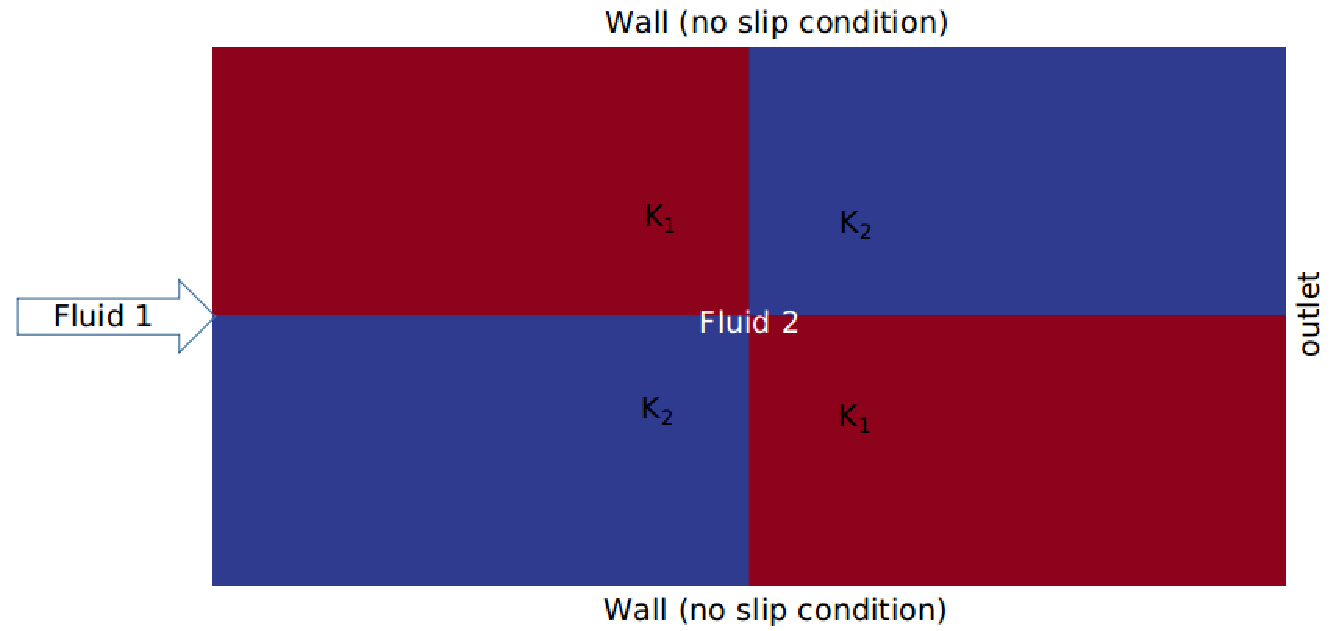
\includegraphics[width=.8\textwidth]{./Pics1/2b2_wi_fine/2b2_whole_in_fine_perm_1.pdf} 
}
\vspace{0.0cm}
\hbox{\hspace{5.0cm} (a) map of permeabilities ($\mathbf{K}$)
}
\vspace{0.25cm}
\hbox{\hspace{1.5cm}
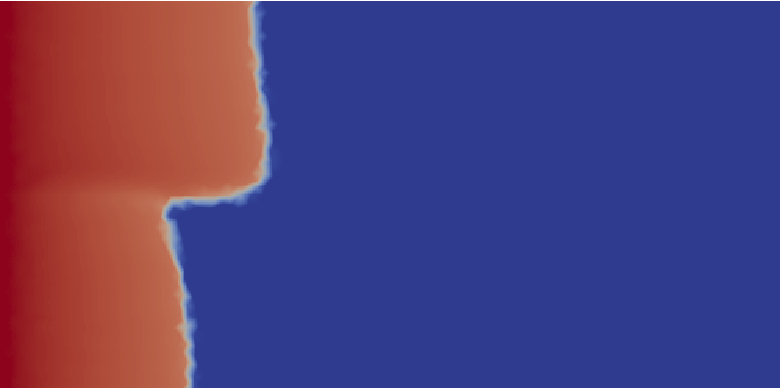
\includegraphics[width=.65\textwidth]{./Pics1/2b2_wi_fine/2b2_whole_in_fine_250_2.pdf}
}
\vspace{0.0cm}
\hbox{\hspace{5.0cm} (b) flow at t=250  \red{(Is this time or the vtu number ??)}
}
\vspace{0.25cm}
\hbox{\hspace{1.5cm}
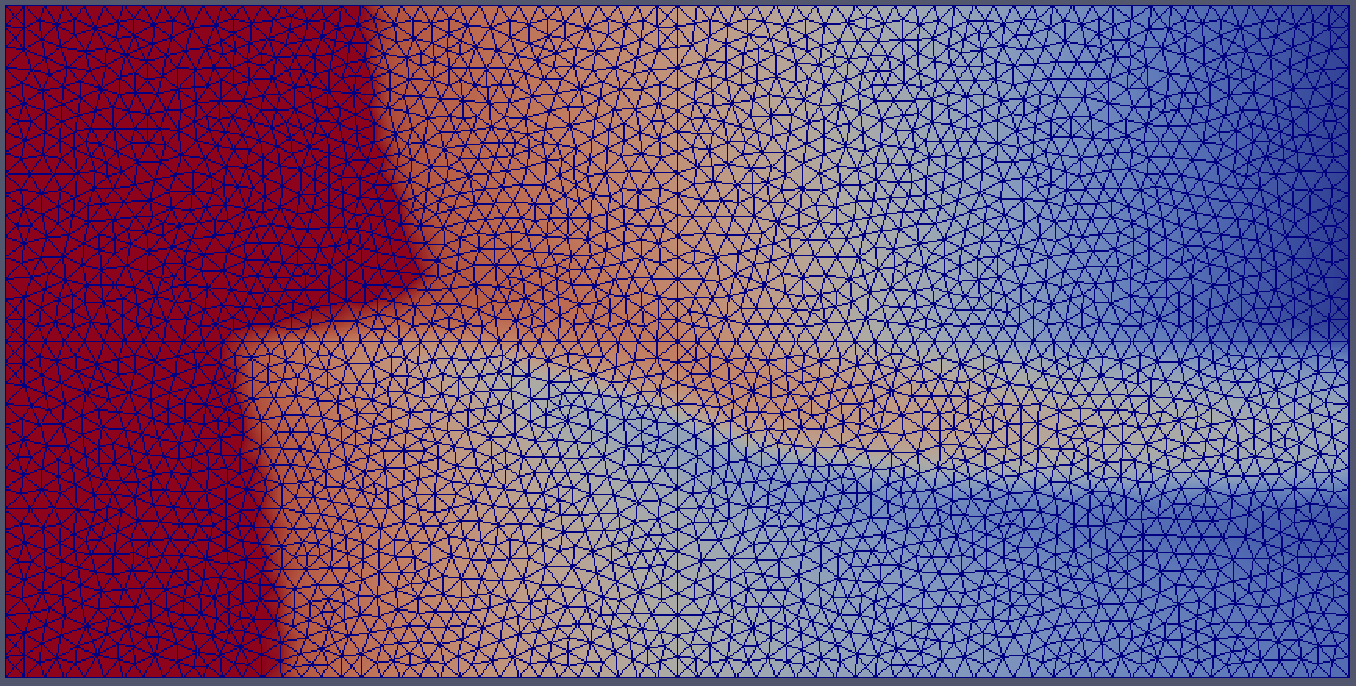
\includegraphics[width=.65\textwidth]{./Pics1/2b2_wi_fine/2b2_whole_in_fine_3000_1.pdf}
}
\vspace{0.0cm}
\hbox{\hspace{5.0cm} (c) flow at t=3000  
}
}     
\caption{Model validation of fluid displacement in heterogeneous porous media: (a) the domain is divided into four subdomains with prescribed synthetic permeability, $\mathbf{K}_{1}=1$ and $\mathbf{K}_{2}=2.5$; (b-c) snapshots of saturation (displacing fluid) field at \red{t=XX} and \red{t=XX}. The domain is discretised in \red{XX} \PN[1]{2} elements. \red{(ALSO YOU MUST ADD SATURATION LEGENDS IN ALL FIGURES.)}}
\label{fem_cv_represent_a}
\end{figure}
\clearpage


%%%
%%% FIGURE
%%%
\begin{landscape}
  \begin{figure}[ht]
    \vbox{ 
      \hbox{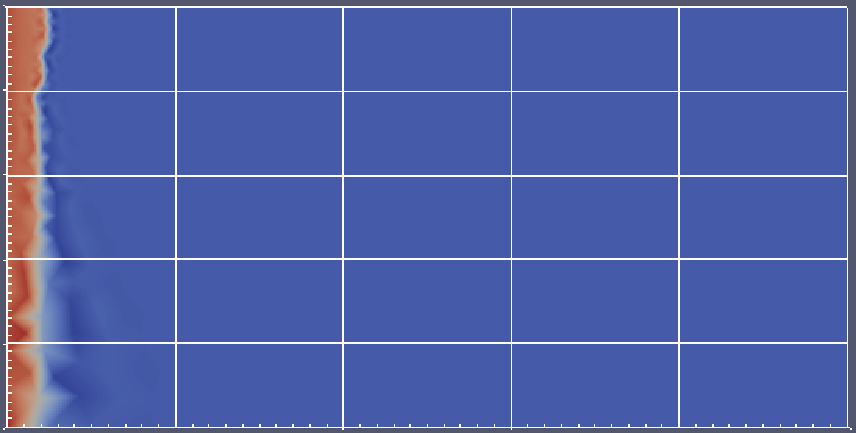
\includegraphics[width=.55\textwidth]{./Pics1/mr1_fixed/mr1_fixed_100_2.pdf}
            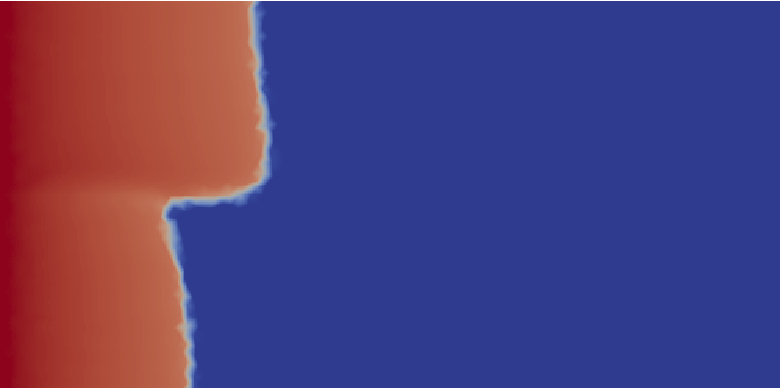
\includegraphics[width=.55\textwidth]{./Pics1/2b2_wi_fine/2b2_whole_in_fine_250_2.pdf}
            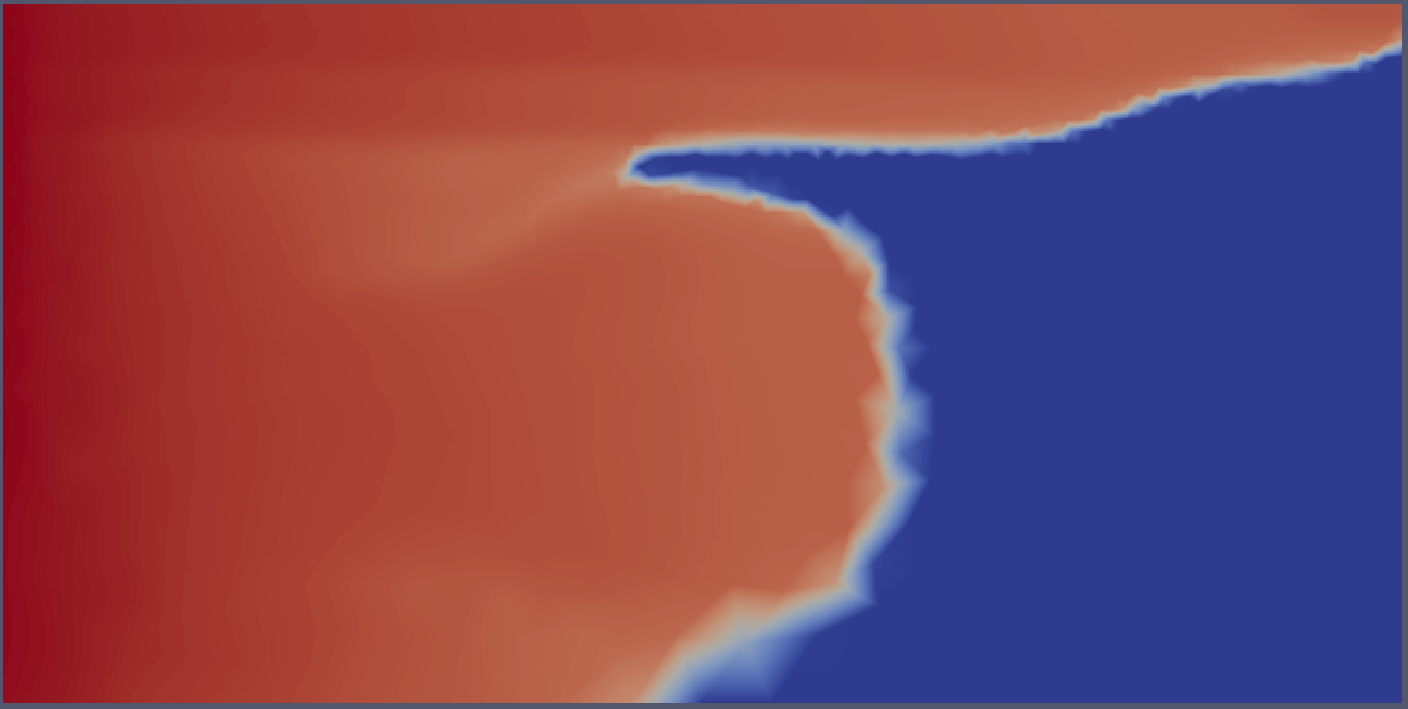
\includegraphics[width=.55\textwidth]{./Pics1/mr1_fixed/mr1_fixed_middle_1.pdf} }
      \vspace{0.cm}
      \hbox{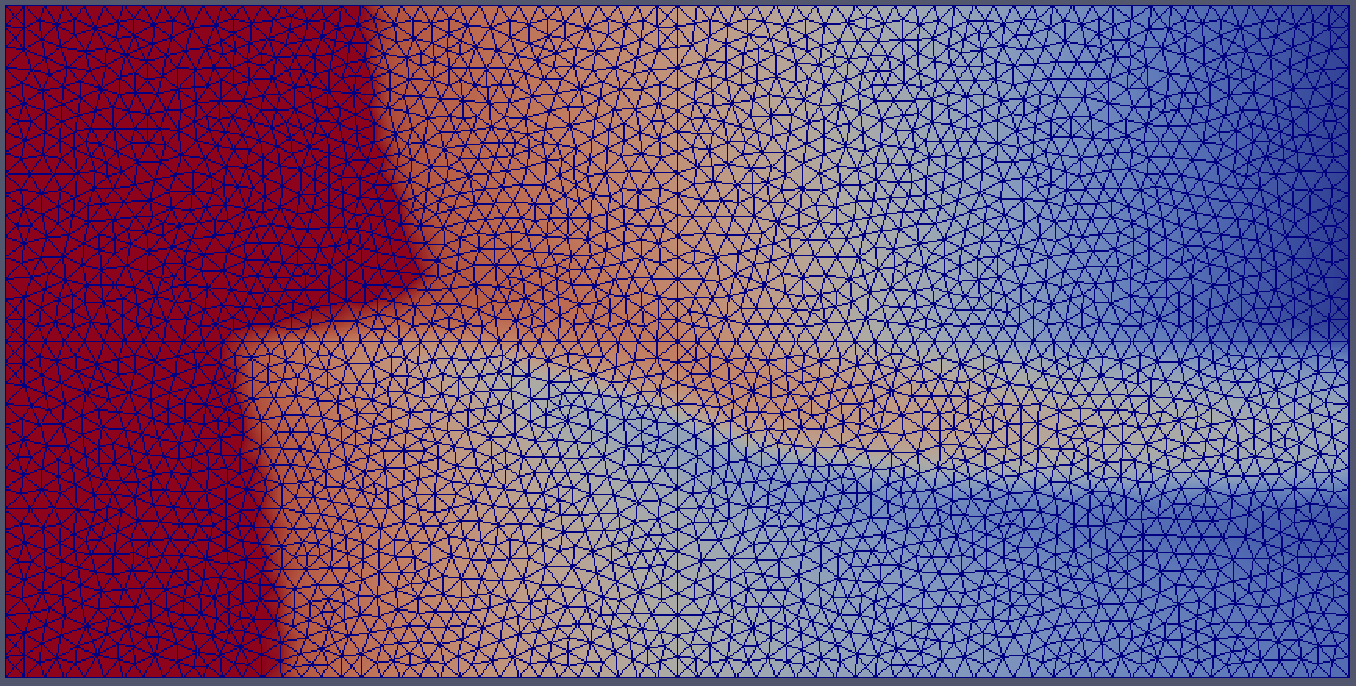
\includegraphics[width=.55\textwidth]{./Pics1/2b2_wi_fine/2b2_whole_in_fine_3000_1.pdf}
            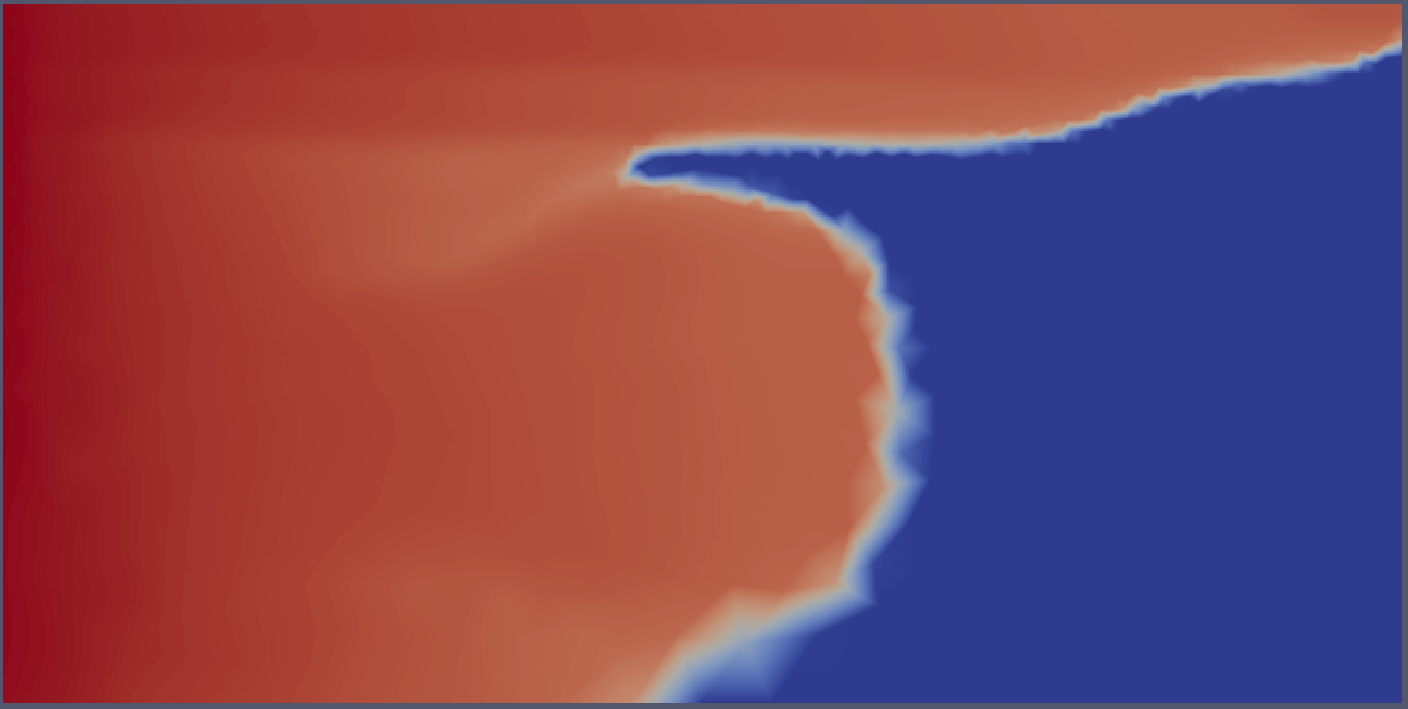
\includegraphics[width=.55\textwidth]{./Pics1/mr1_fixed/mr1_fixed_middle_1.pdf}}}
\caption{\red{THIS IS JUST FOR OUR OWN COMPARISON ... IT DOESN'T SEEM TO MATCH ... }}
\label{fem_cv_represent_abc}
\end{figure}
\end{landscape}
\clearpage
%%%
%%%
%%%



%%%
%%% FIGURE
%%%
\begin{landscape}
  \begin{figure}[ht]
    \vbox{ 
      \hbox{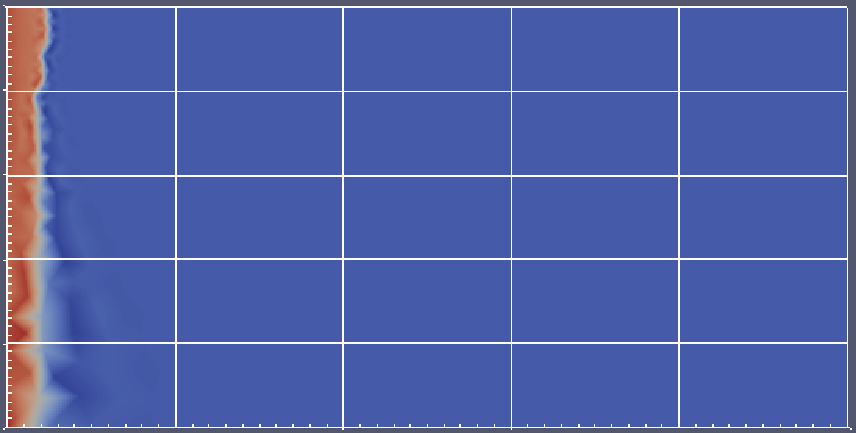
\includegraphics[width=.55\textwidth]{./Pics1/mr1_fixed/mr1_fixed_100_2.pdf}
            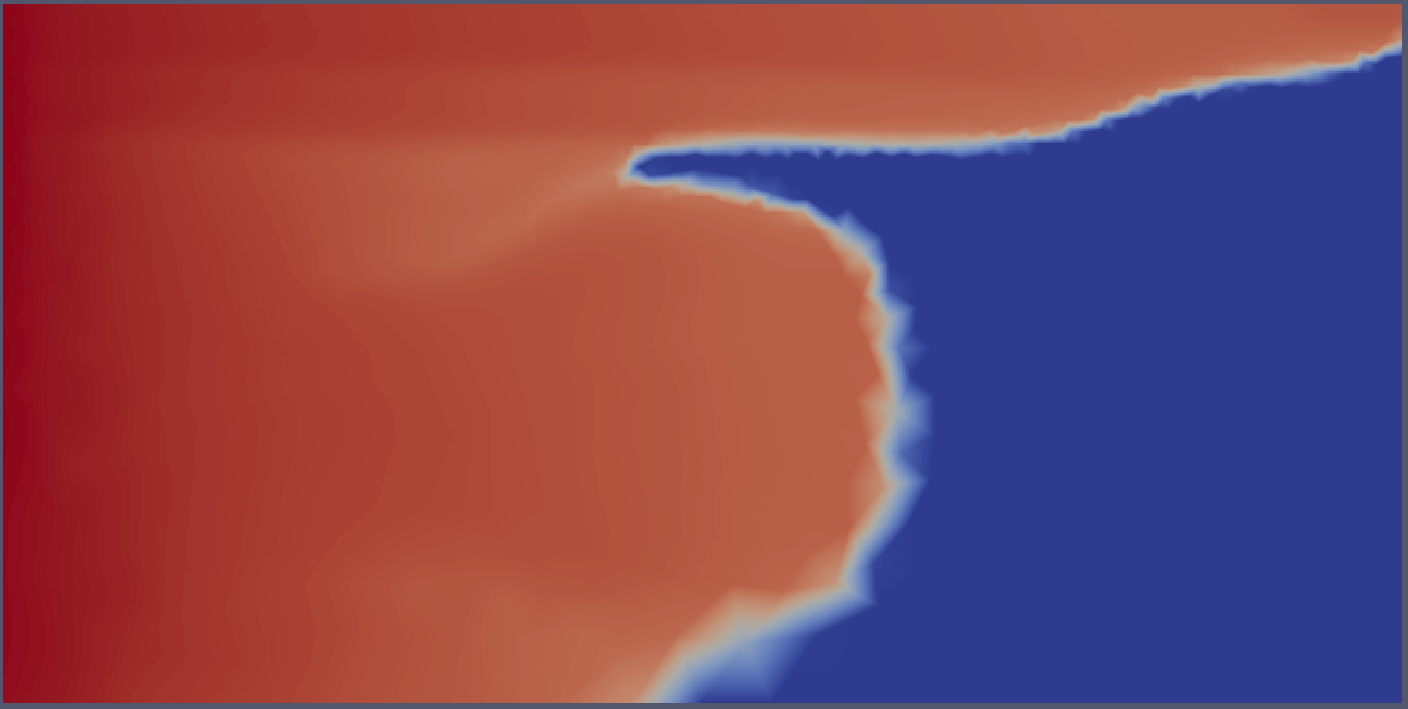
\includegraphics[width=.55\textwidth]{./Pics1/mr1_fixed/mr1_fixed_middle_1.pdf} 
            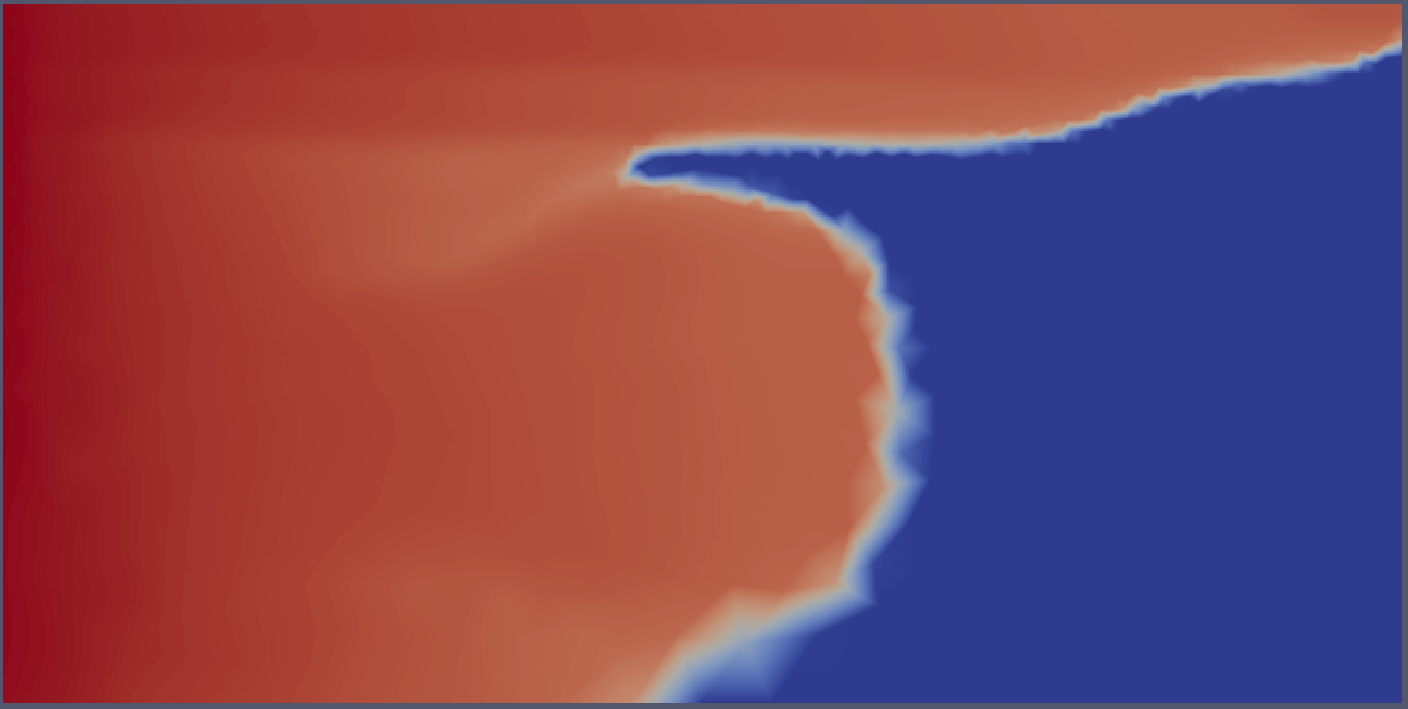
\includegraphics[width=.55\textwidth]{./Pics1/mr1_fixed/mr1_fixed_middle_1.pdf} }
      \hbox{\hspace{10cm} (a) VR = 1}
      \vspace{1cm}
      \hbox{
\includegraphics[width=.55\textwidth]{./Pics1/mr10_fixed/mr10_fixed_100_1.pdf}
            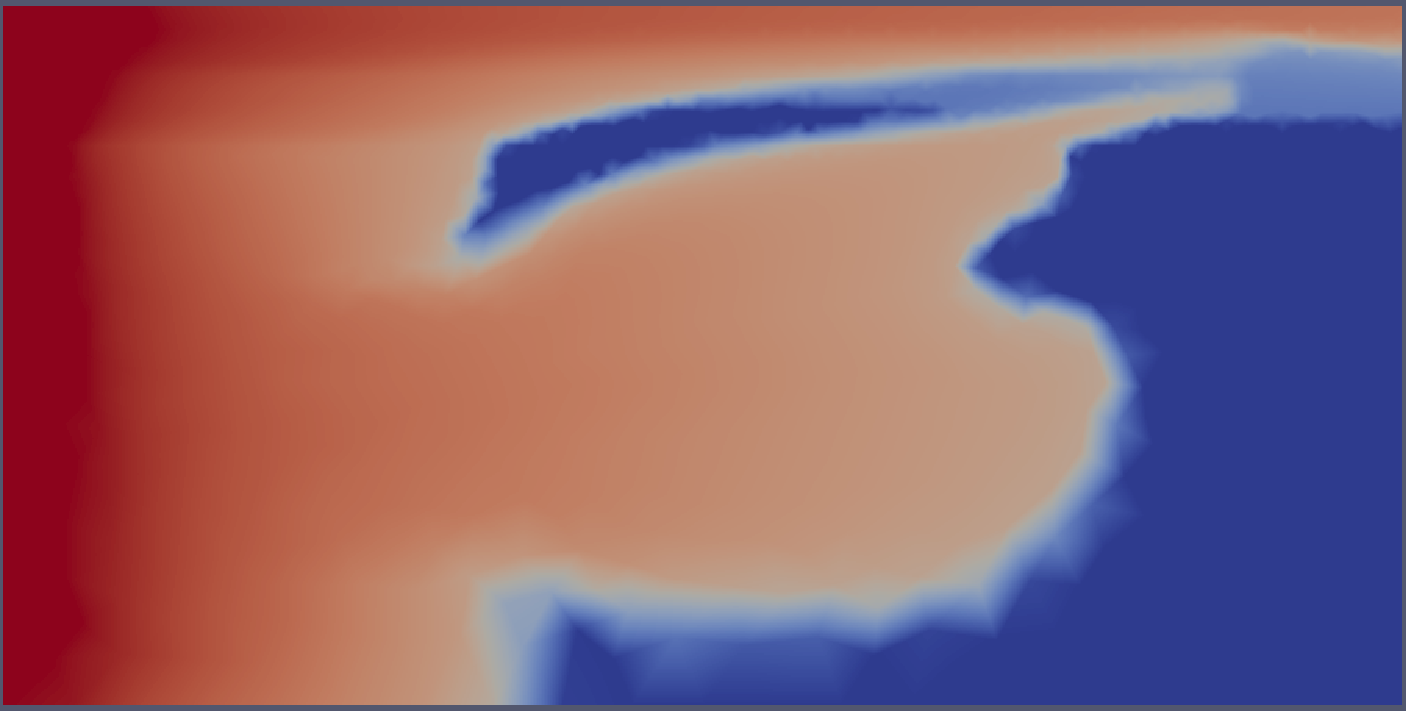
\includegraphics[width=.55\textwidth]{./Pics1/mr10_fixed/mr10_fixed_middle_1.pdf}
            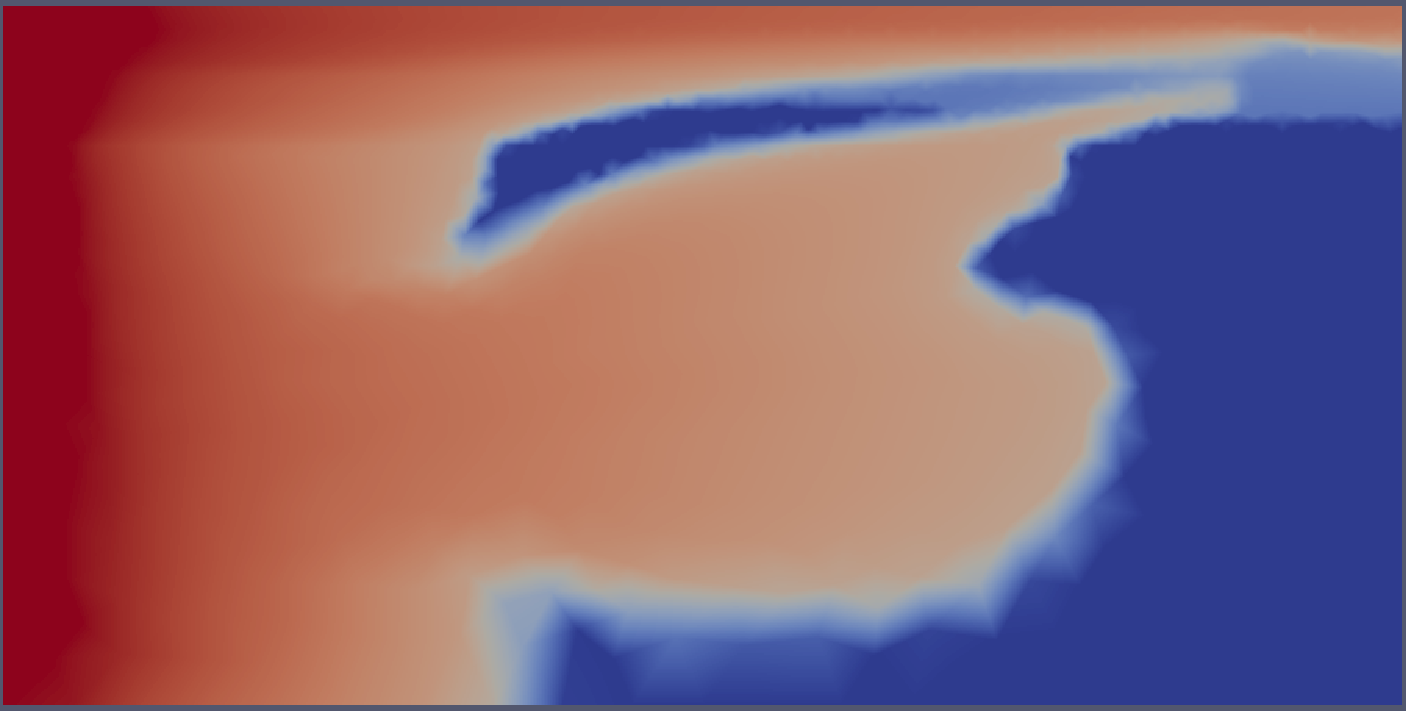
\includegraphics[width=.55\textwidth]{./Pics1/mr10_fixed/mr10_fixed_middle_1.pdf} }
      \hbox{\hspace{10cm} (b) VR = 10  }}
\caption{Initial model validation: snapshots of numerical simulations performed with VR=1 and VR=10 (the domain contains \red{XX} elements). \red{(It is clear that figures are not correct ... as they seem wrong.)}}
\label{fem_cv_represent_a}
\end{figure}
\end{landscape}
\clearpage
%%%
%%%
%%%



%%%%
%%%%  FIGURE
%%%%
\begin{figure}[ht] 
\vbox{
\hbox{\hspace{1.5cm}
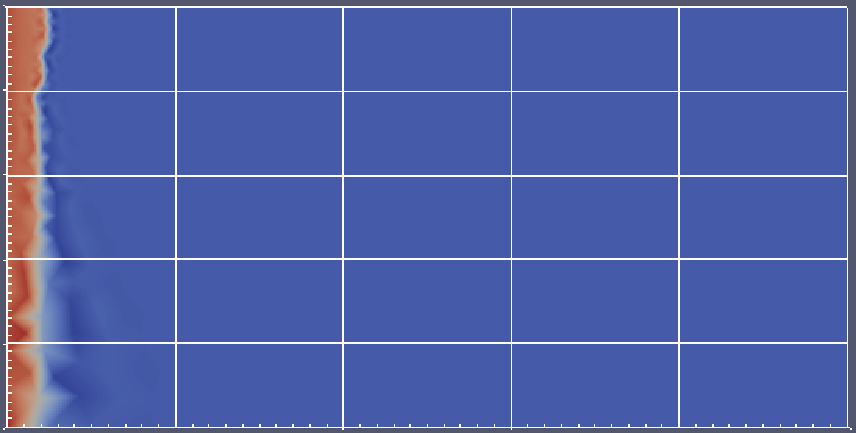
\includegraphics[width=.85\textwidth]{./Pics1/mr1_fixed/mr1_fixed_100_2.pdf} 
}
\vspace{0.0cm}
\hbox{\hspace{4.0cm} (a) MR1 at t = 100 (start)   
}
\vspace{0.25cm}
\hbox{\hspace{1.5cm}

\includegraphics[width=.85\textwidth]{./Pics1/mr10_fixed/mr10_fixed_100_1.pdf}
}
\vspace{0.0cm}
\hbox{\hspace{4.0cm} (b) MR10 at t = 100 (start)  
}
}     
\caption{Comparing the the MR1 and MR10 cases using fixed mesh in the beggining of the simulation.}
\label{fig:6a}
\end{figure}
\clearpage

%%%%
%%%%  FIGURE
%%%%
\begin{figure}[ht] 
\vbox{
\hbox{\hspace{1.5cm}
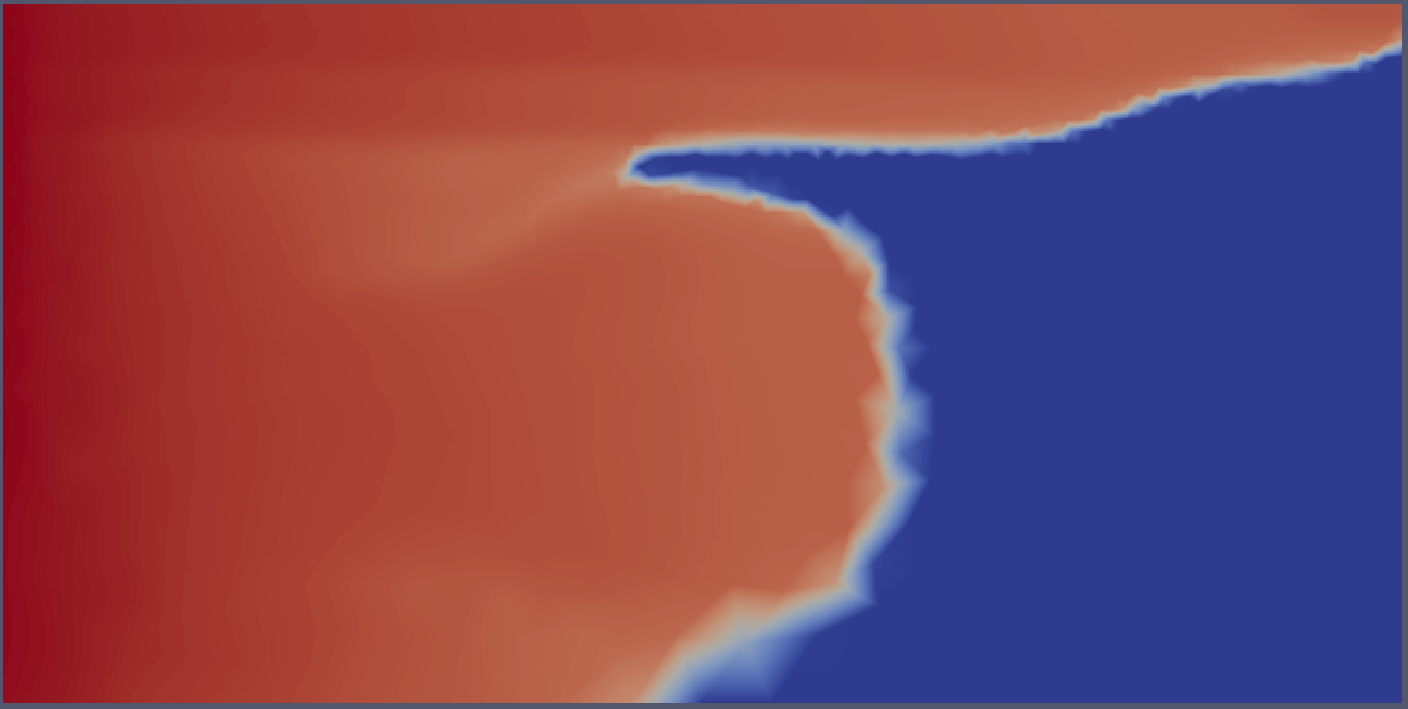
\includegraphics[width=.85\textwidth]{./Pics1/mr1_fixed/mr1_fixed_middle_1.pdf} 
}
\vspace{0.0cm}
\hbox{\hspace{4.0cm} (a) MR1 at t = 1500 (middle)   
}
\vspace{0.25cm}
\hbox{\hspace{1.5cm}
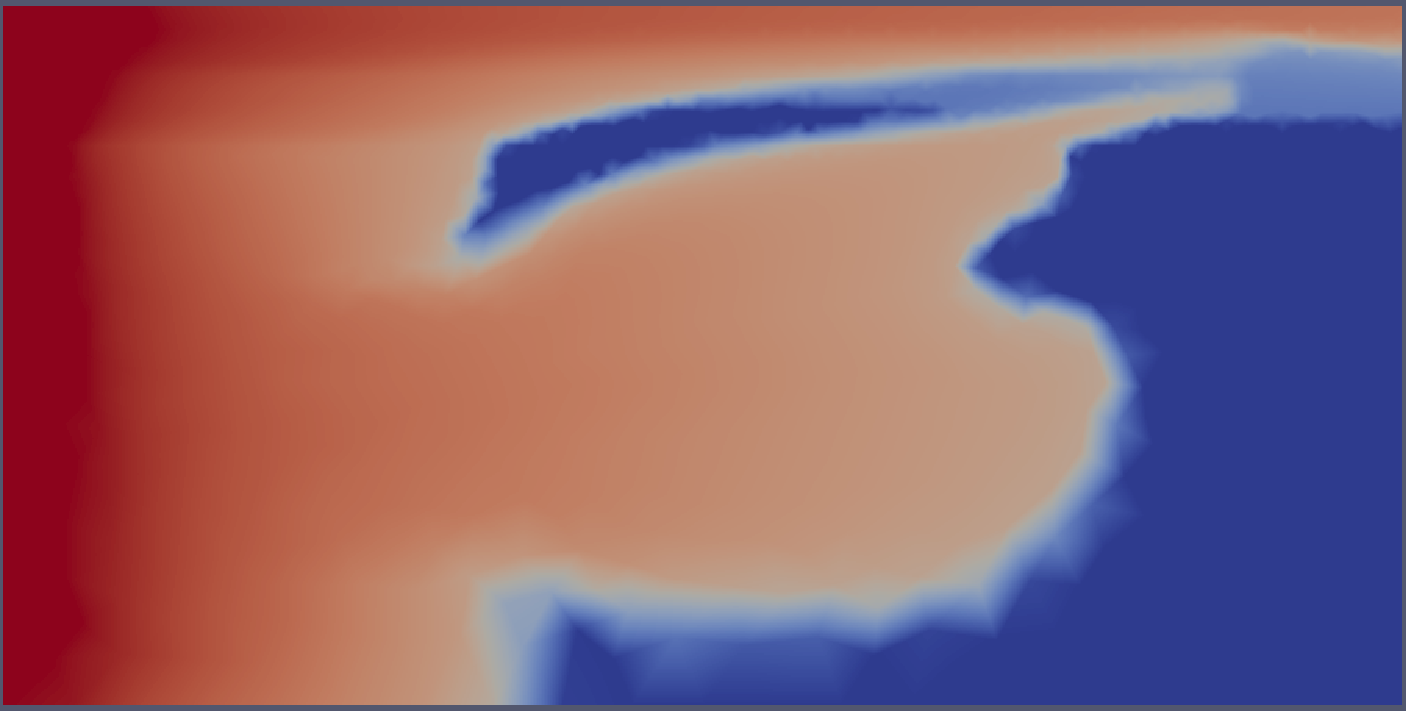
\includegraphics[width=.85\textwidth]{./Pics1/mr10_fixed/mr10_fixed_middle_1.pdf}
}
\vspace{0.0cm}
\hbox{\hspace{4.0cm} (b) MR10 at t = 1500 (middle)  
}
}     
\caption{Comparing the the MR1 and MR10 cases using fixed mesh in the middle of the simulation.}
\label{fig:6b}
\end{figure}
\clearpage

%%%%
%%%%  FIGURE
%%%%
\begin{figure}[ht] 
\vbox{
\hbox{\hspace{1.5cm}
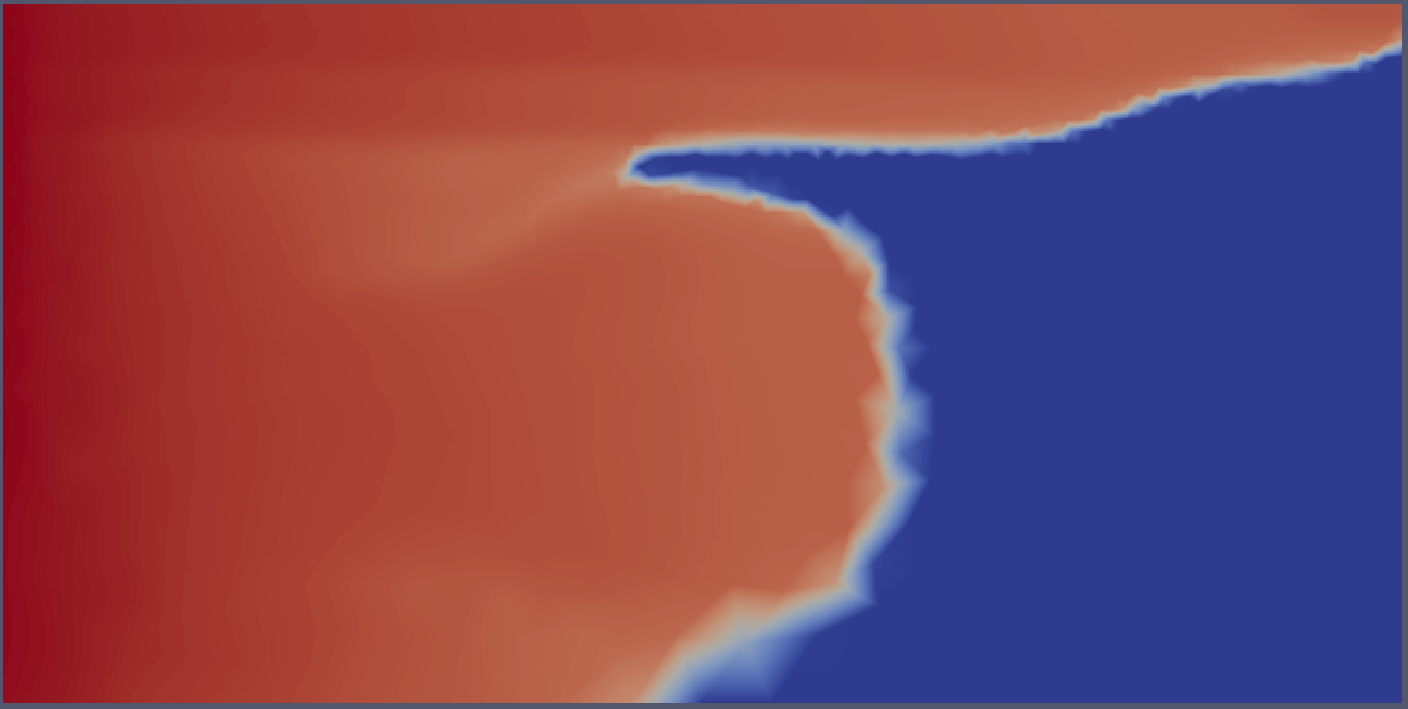
\includegraphics[width=.85\textwidth]{./Pics1/mr1_fixed/mr1_fixed_middle_1.pdf} 
}
\vspace{0.0cm}
\hbox{\hspace{4.0cm} (a) MR1 at t = 3000 (end)   
}
\vspace{0.25cm}
\hbox{\hspace{1.5cm}
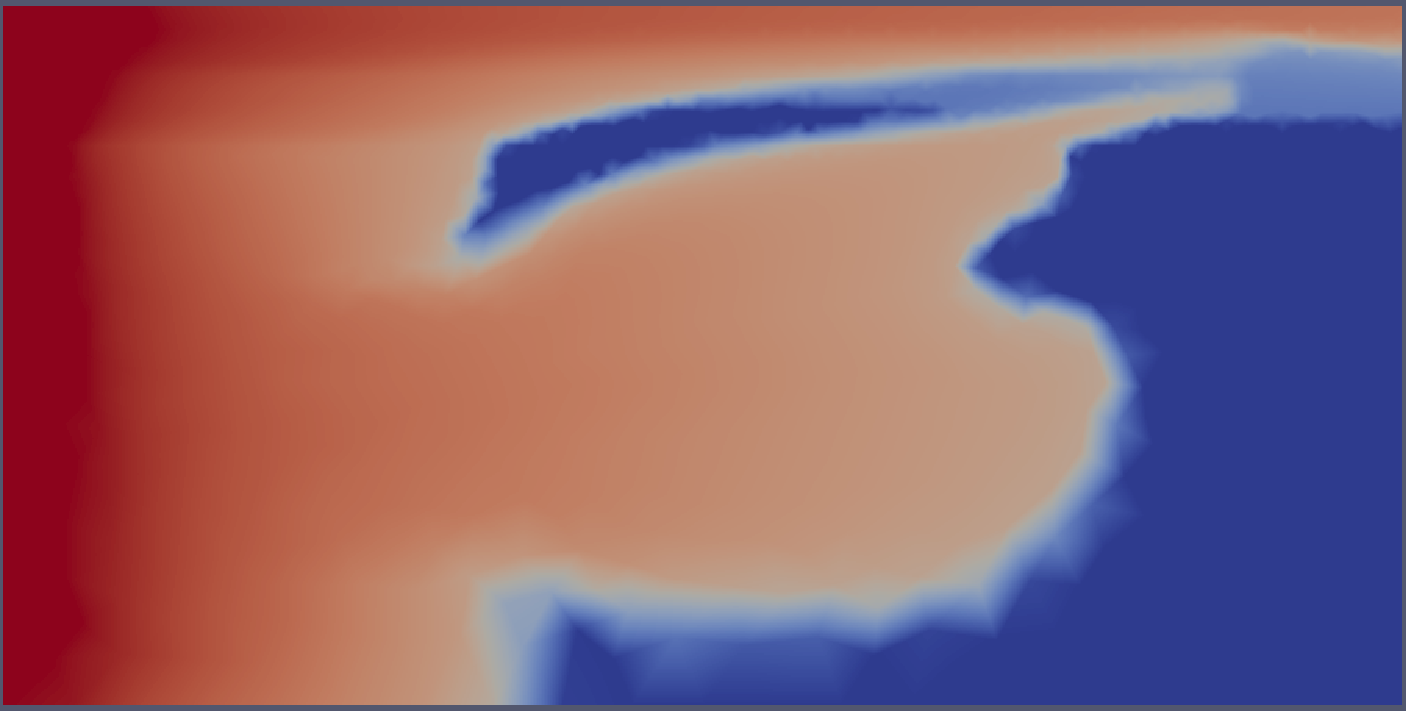
\includegraphics[width=.85\textwidth]{./Pics1/mr10_fixed/mr10_fixed_middle_1.pdf}
}
\vspace{0.0cm}
\hbox{\hspace{4.0cm} (b) MR10 at t = 3000 (end)  
}
}     
\caption{Comparing the the MR1 and MR10 cases using fixed mesh in the end of the simulation.}
\label{fig:6c}
\end{figure}
\clearpage


%%%%
%%%%  FIGURE
%%%%
\begin{landscape}
\begin{figure}[ht] 
\vbox{\vspace{-1cm}
\hbox{\includegraphics[width=.5\textwidth]{./Pics1/Saffman_homogeneous_MR3/saffman_homo_fixed_1.pdf}
      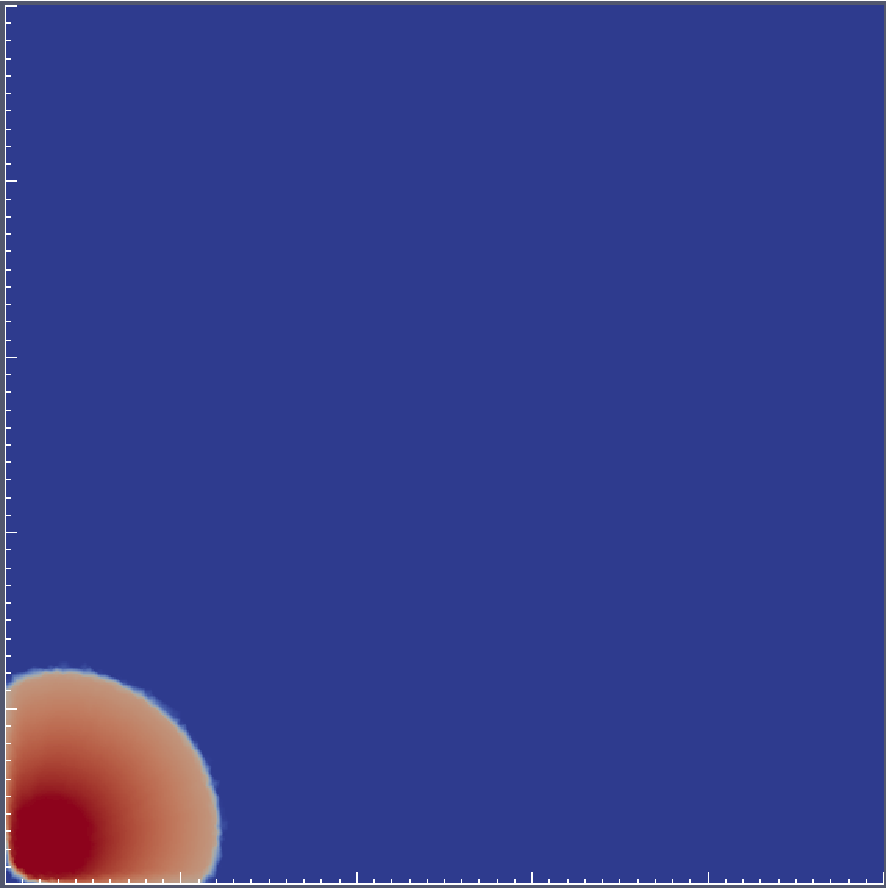
\includegraphics[width=.5\textwidth]{./Pics1/Saffman_homogeneous_MR3/saffman_homo_fixed_250.pdf}
      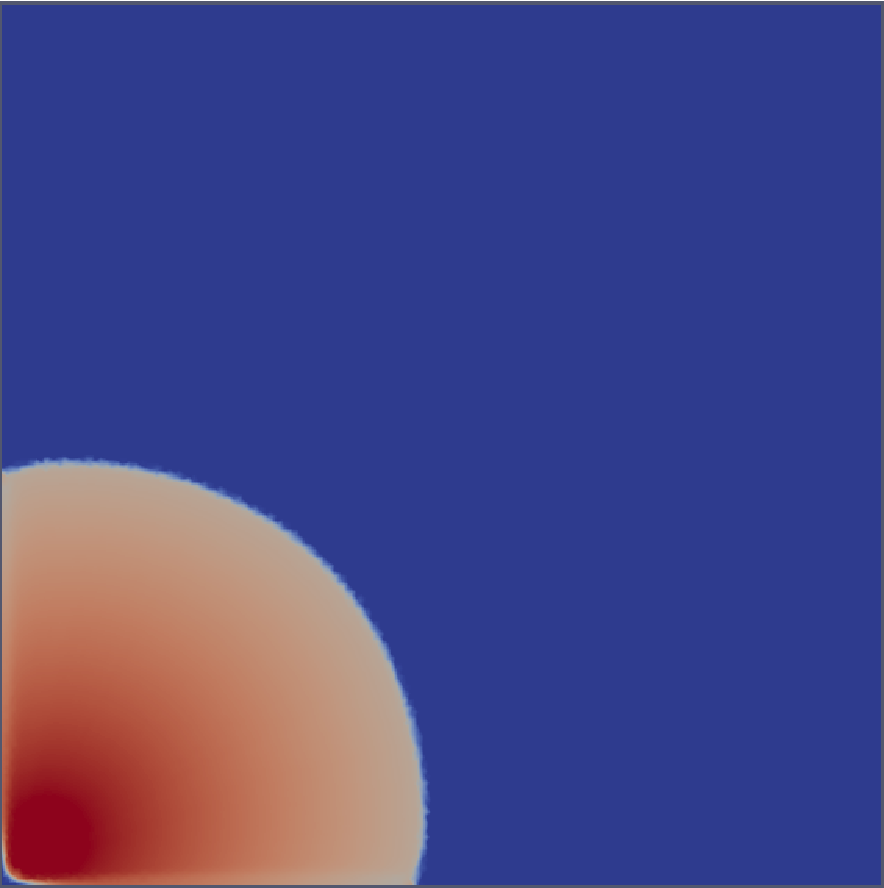
\includegraphics[width=.5\textwidth]{./Pics1/Saffman_homogeneous_MR3/saffman_homo_fixed_1000.pdf}}
\vspace{0.cm}
\hbox{\hspace{1.0cm} (a) pressure at t=0 \hspace{3.cm} (b) t=250\red{(???)} \hspace{3.0cm} (c) t=1000\red{(???)}}
\vspace{0.5cm}
\hbox{
      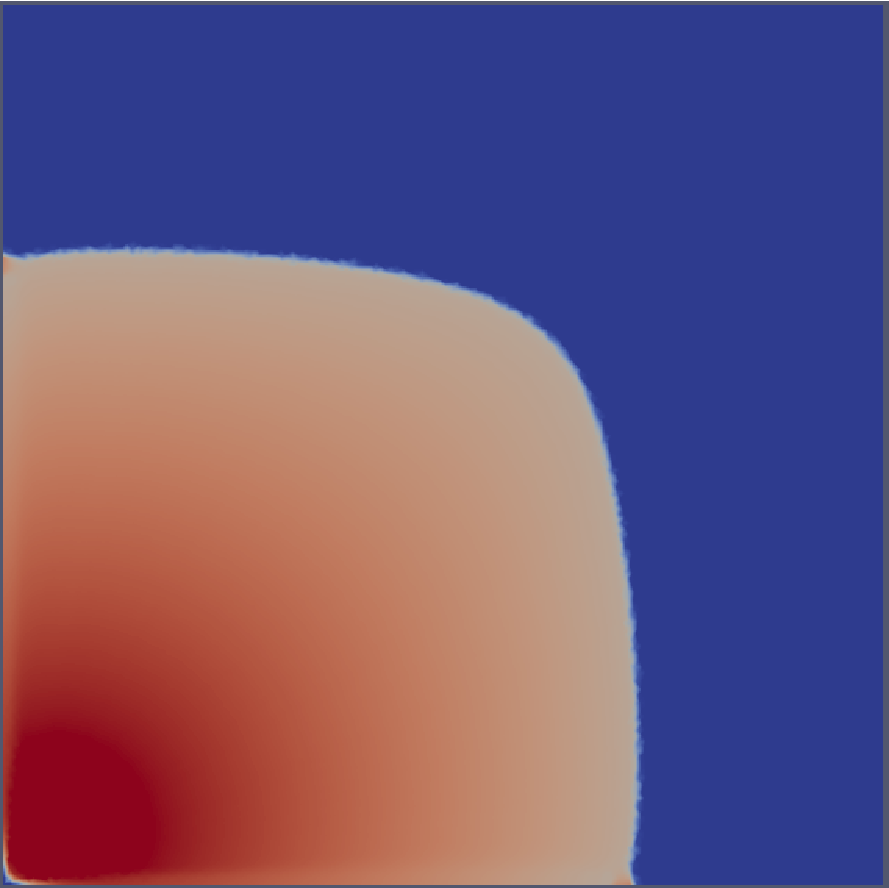
\includegraphics[width=.5\textwidth]{./Pics1/Saffman_homogeneous_MR3/saffman_homo_fixed_2500.pdf}
      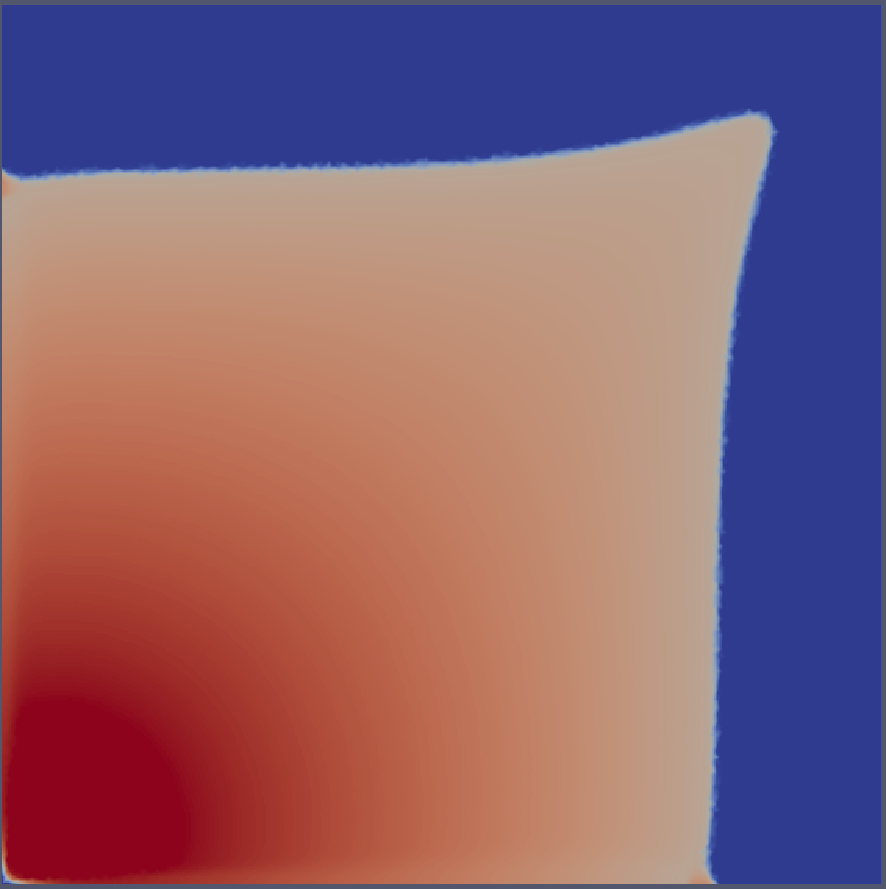
\includegraphics[width=.5\textwidth]{./Pics1/Saffman_homogeneous_MR3/saffman_homo_fixed_3500.pdf} 
      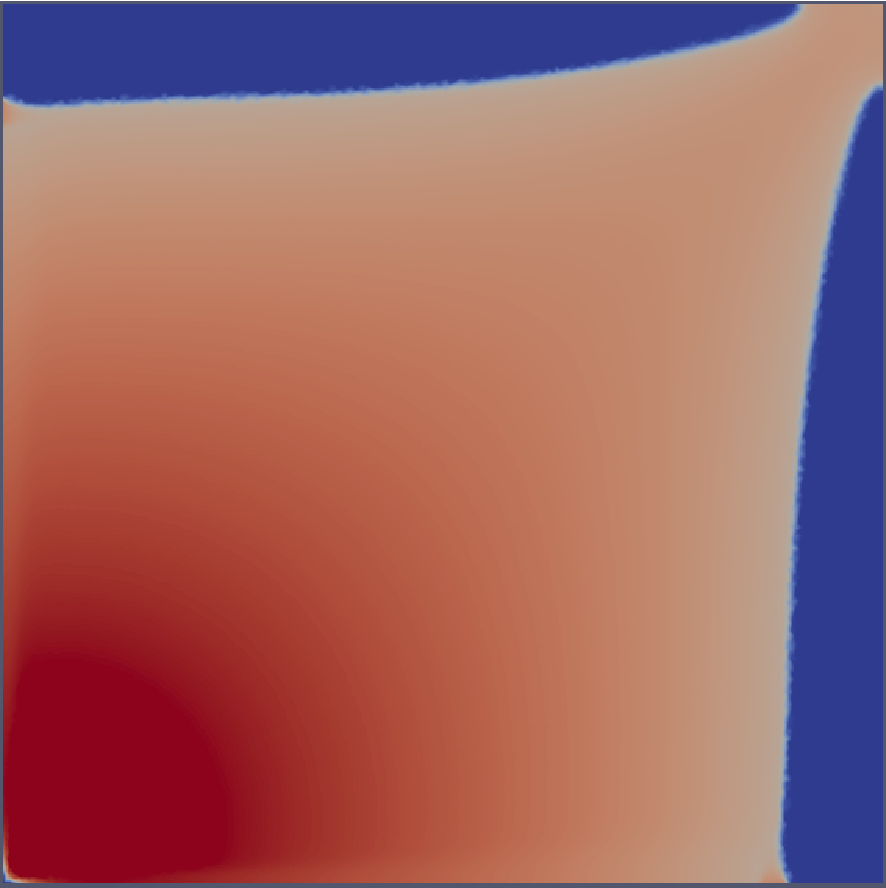
\includegraphics[width=.5\textwidth]{./Pics1/Saffman_homogeneous_MR3/saffman_homo_fixed_end_1.pdf}}
\vspace{0.cm}
\hbox{ \hspace{2.cm} (d) t=2500\red{(???)} \hspace{3.0cm} (e) t=1000\red{(???)}   \hspace{4.cm} (f) t=XXX\red{(???)}}
\vspace{0.cm}
}   
\caption{Simulated flow in a Hele-Shaw cell ({\it VR}=3): (a) pressure profile \red{(is it true?}) $\left(\text{in g.cm}^{-1}\text{.s}^{-2}\right)$ with source and sink regions are explicitly shown along with dimensions (in cm); (b-f) snapshots of wetting phase saturation showing flow profile as the simulation evolves. The domain contains \red{XX} \PN[1]{2} triangular elements. \red{(ADD SATURATION AND PRESSURE LEGENDS !!)}}
\label{fig:homoheleshaw_VN3}
\end{figure}
\end{landscape}
\clearpage


%%%%
%%%%  FIGURE
%%%%
\begin{landscape}
\begin{figure}[ht] 
\vbox{\vspace{-1cm}
\hbox{\includegraphics[width=.5\textwidth]{./Pics1/Saffman_homogeneous/saffman_homo_fixed_1.pdf}
      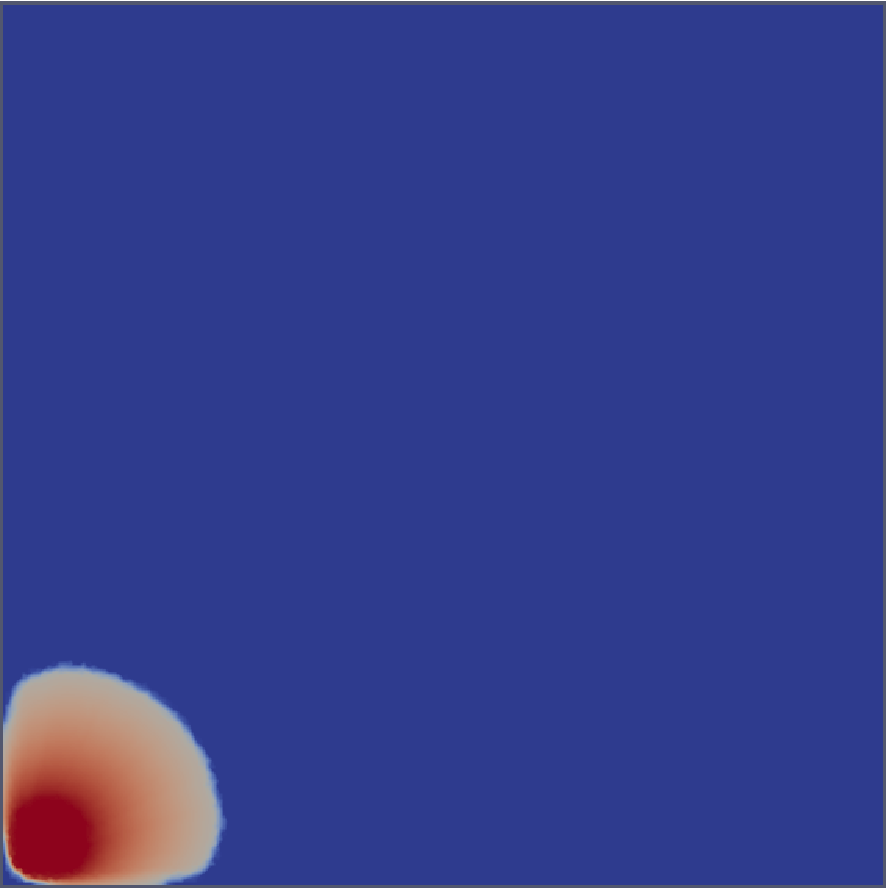
\includegraphics[width=.5\textwidth]{./Pics1/Saffman_homogeneous/saffman_homo_fixed_250_1.pdf}
      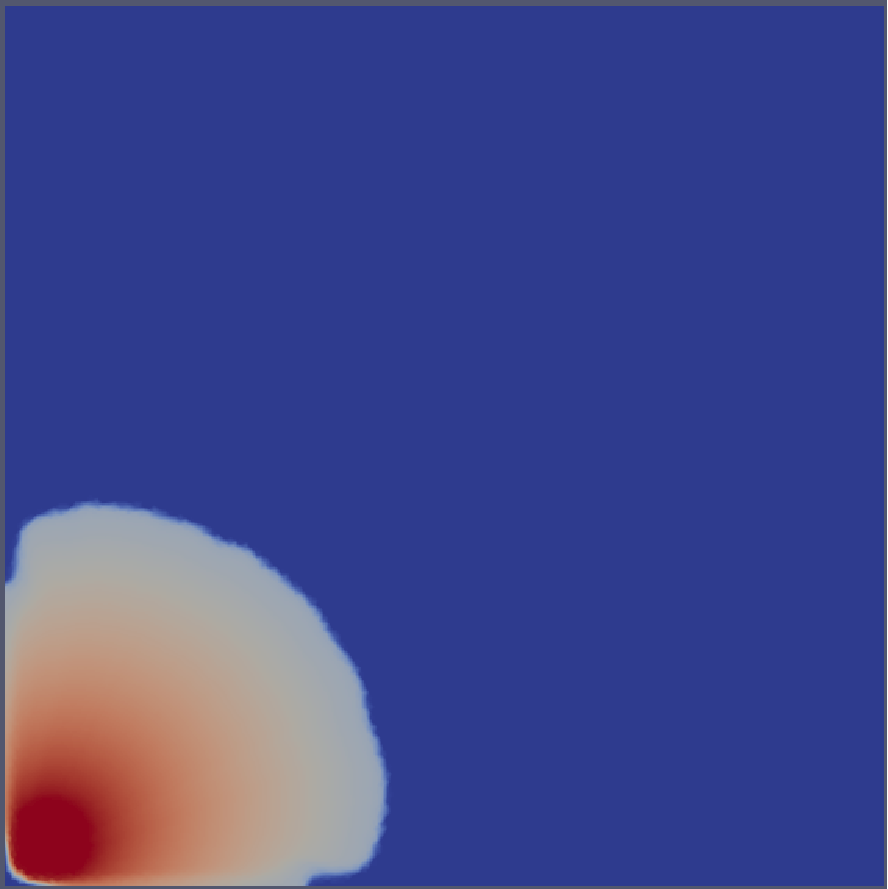
\includegraphics[width=.5\textwidth]{./Pics1/Saffman_homogeneous/saffman_homo_fixed_1000.pdf}}
\vspace{0.cm}
\hbox{\hspace{1.0cm} (a) pressure at t=0 \hspace{3.cm} (b) t=250\red{(???)} \hspace{3.0cm} (c) t=1000\red{(???)}}
\vspace{0.5cm}
\hbox{
      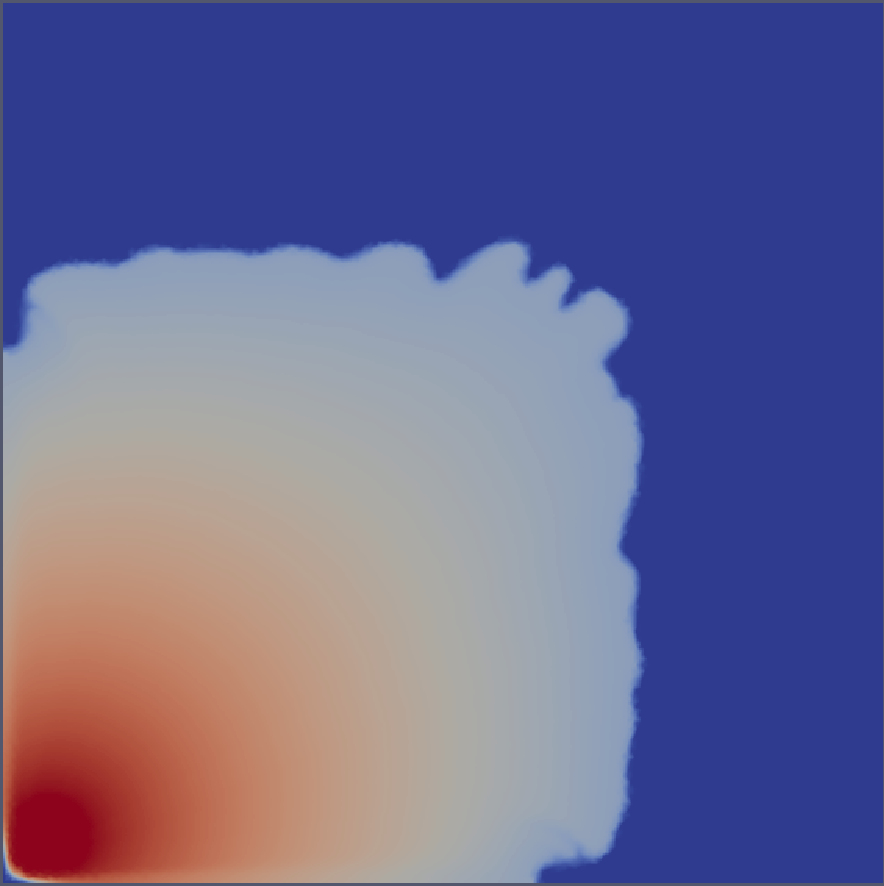
\includegraphics[width=.5\textwidth]{./Pics1/Saffman_homogeneous/saffman_homo_fixed_6000.pdf}
      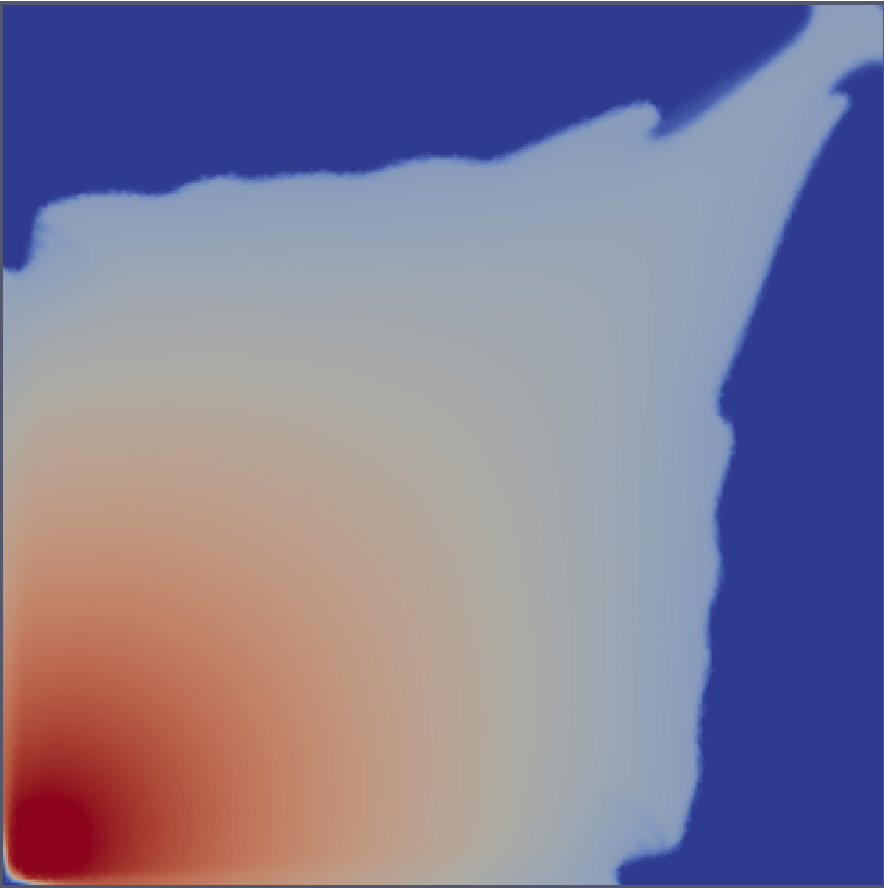
\includegraphics[width=.5\textwidth]{./Pics1/Saffman_homogeneous/saffman_homo_fixed_end_1.pdf}}
\vspace{0.cm}
\hbox{ \hspace{2.cm} (d) t=6000\red{(???)} \hspace{4.cm} (e) t=XXX\red{(???)}}
\vspace{0.cm}
}   
\caption{Simulated flow in a Hele-Shaw cell ({\it VR}=10): (a) pressure profile \red{(is it true?}) $\left(\text{in g.cm}^{-1}\text{.s}^{-2}\right)$ with source and sink regions explicitly shown along with dimensions (in cm); (b-e) snapshots of wetting phase saturation showing flow profile as the simulation evolves. The domain contains \red{XX} \PN[1]{2} triangular elements. \red{(ADD SATURATION AND PRESSURE LEGENDS !! ... IF THE LEGENDS ARE THE SAME AS IN THE PREVIOUS PIC, THEN JUST EXPLICITLY REFER TO THEM)}}
\label{fig:homoheleshaw_VN10}
\end{figure}
\end{landscape}
\clearpage



%%%%
%%%%  FIGURE
%%%%
\begin{figure}[ht] 
\vbox{
\hbox{\hspace{2.5cm}
\includegraphics[width=.6\textwidth]{./Pics1/Saffman_homogeneous_MR3/saffman_homo_fixed_1.pdf} 
}
\vspace{0.0cm}
\hbox{\hspace{4.0cm} (a) Hell-Shaw cell domain   
}
\vspace{0.25cm}
\hbox{\hspace{2.5cm}
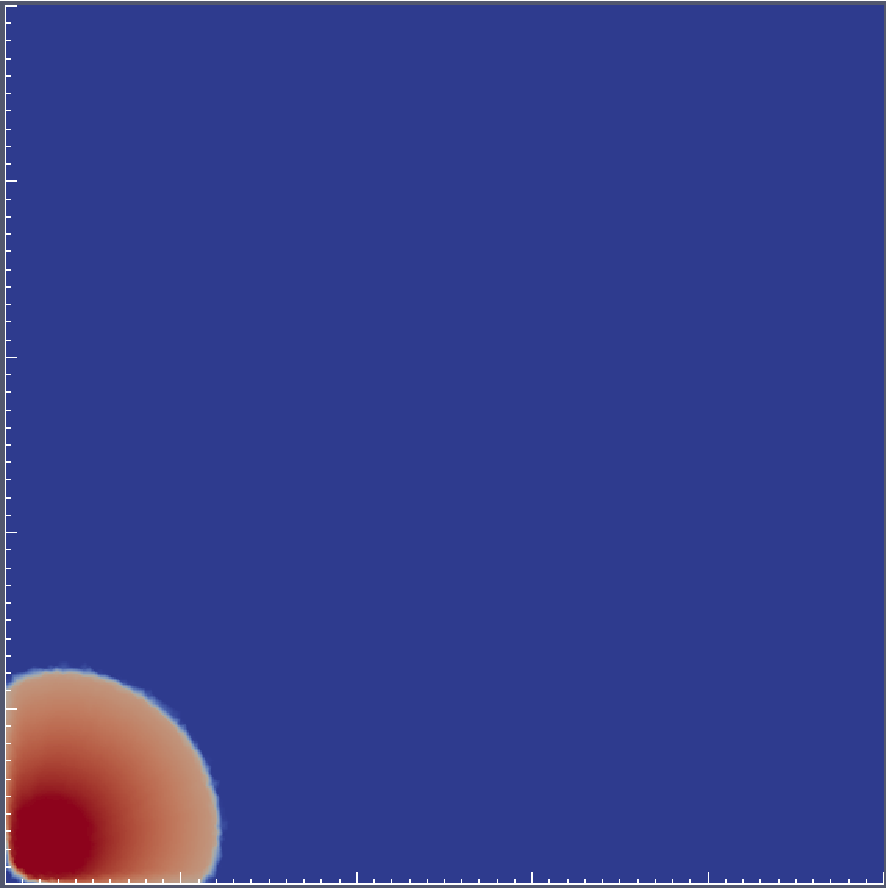
\includegraphics[width=.6\textwidth]{./Pics1/Saffman_homogeneous_MR3/saffman_homo_fixed_250.pdf}
}
\vspace{0.0cm}
\hbox{\hspace{5.0cm} (b) flow at t=250  
}
}     
\caption{This is a description of a Hele-Shaw experimental domain, showing the source and sink term as this is implied in this test-case followed by a screenshot of the flow at time, t=250(b). More screenshot follow that describe the progression of the flow in figure \ref{fig:1b_homoheleshaw_3} and figure \ref{fig:1c_homoheleshaw_3}.}
\label{fig:1a_homoheleshaw_3}
\end{figure}
\clearpage

%%%%
%%%%  FIGURE
%%%%
\begin{figure}[ht] 
\vbox{
\hbox{\hspace{2.5cm}
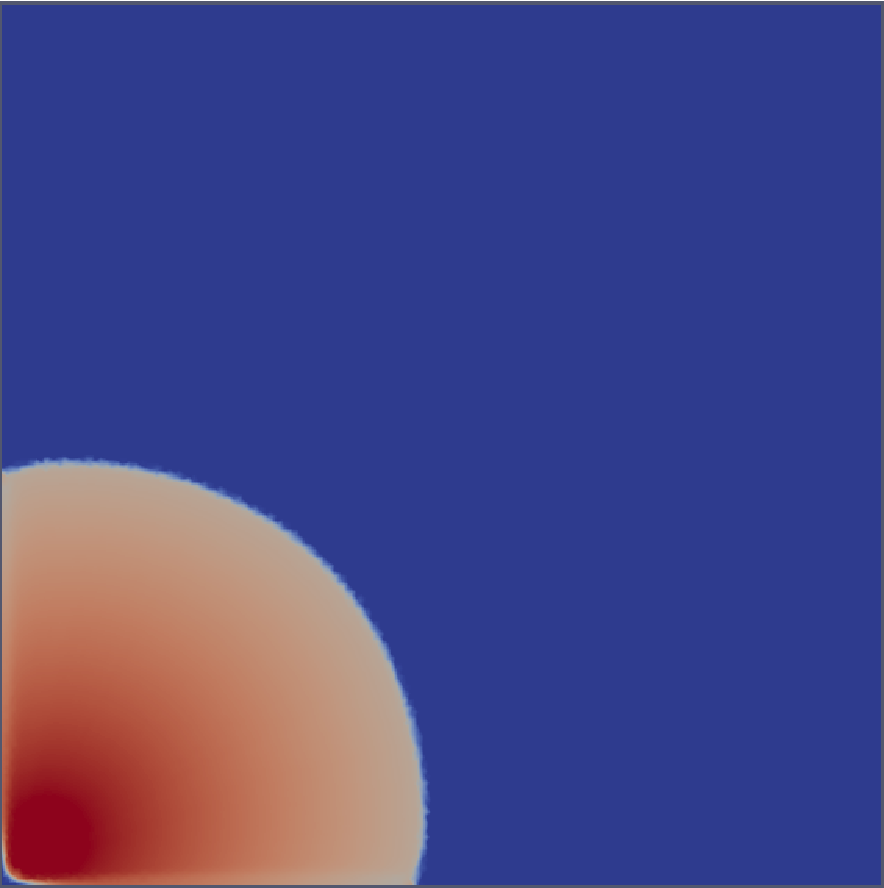
\includegraphics[width=.6\textwidth]{./Pics1/Saffman_homogeneous_MR3/saffman_homo_fixed_1000.pdf} 
}
\vspace{0.0cm}
\hbox{\hspace{5.0cm} (a) flow at t=1000   
}
\vspace{0.25cm}
\hbox{\hspace{2.5cm}
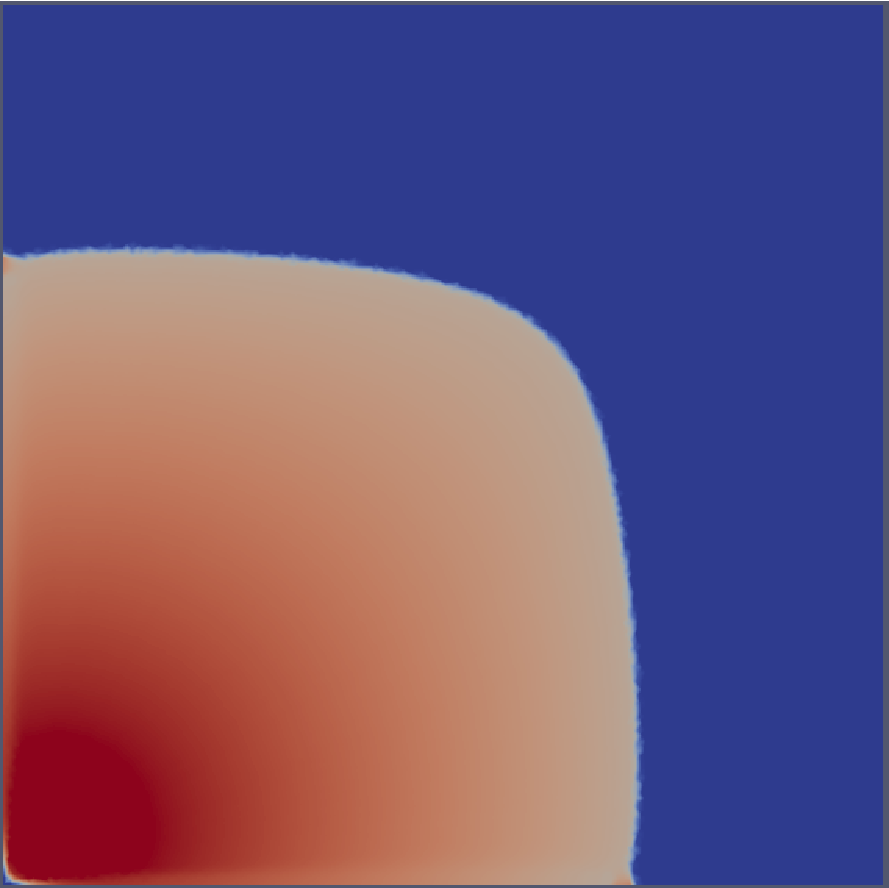
\includegraphics[width=.6\textwidth]{./Pics1/Saffman_homogeneous_MR3/saffman_homo_fixed_2500.pdf}
}
\vspace{0.0cm}
\hbox{\hspace{5.0cm} (b) flow at t=2500  
}
}     
\caption{Following figure \ref{fig:1a_homoheleshaw_3} as the flow progress, t=1000(a), a tip start to appears, at t=2500(b).}
\label{fig:1b_homoheleshaw_3}
\end{figure}
\clearpage

%%%%
%%%%  FIGURE
%%%%
\begin{figure}[ht] 
\vbox{
\hbox{\hspace{2.5cm}
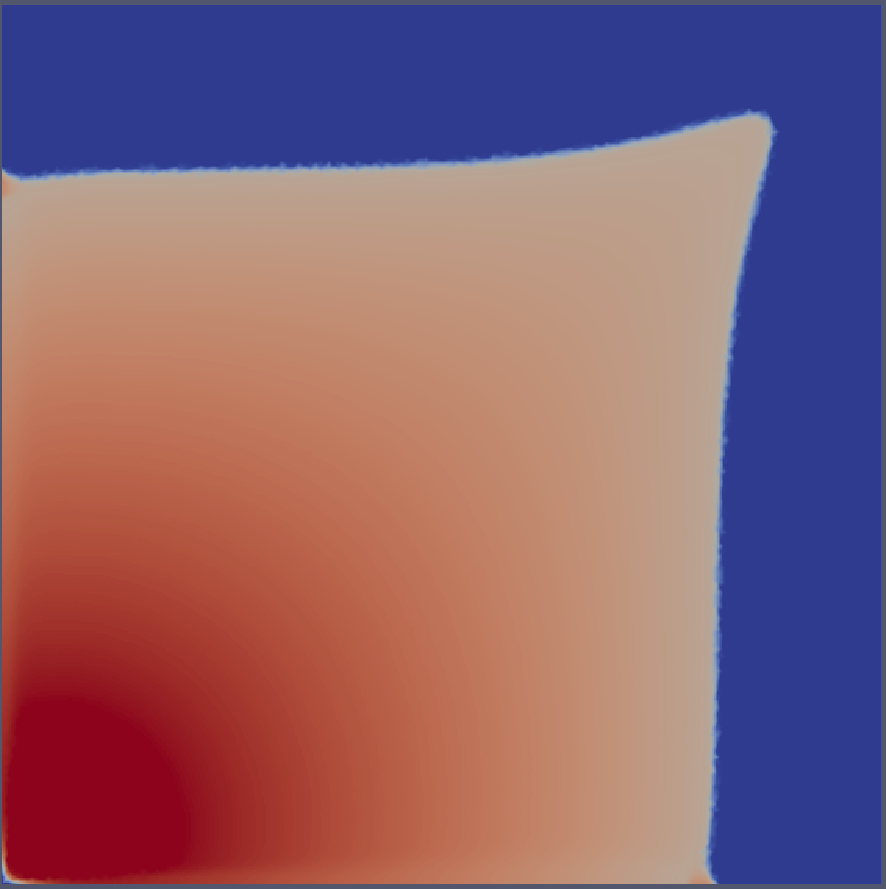
\includegraphics[width=.6\textwidth]{./Pics1/Saffman_homogeneous_MR3/saffman_homo_fixed_3500.pdf} 
}
\vspace{0.0cm}
\hbox{\hspace{5.0cm} (a) flow at t=3500   
}
\vspace{0.25cm}
\hbox{\hspace{2.5cm}
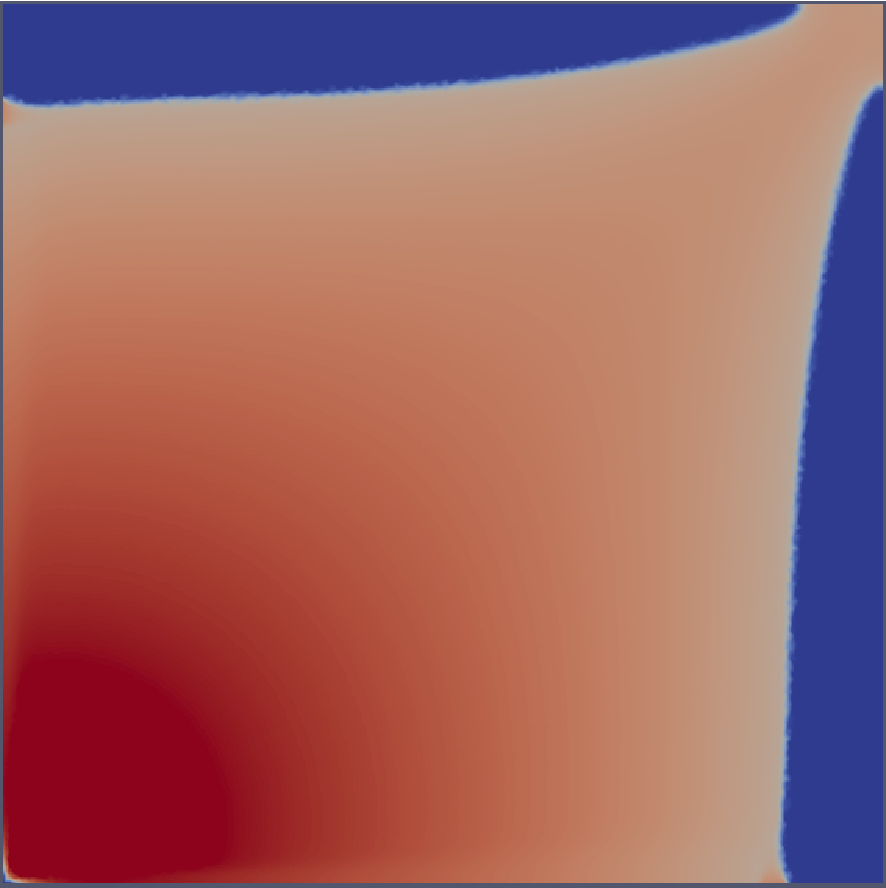
\includegraphics[width=.6\textwidth]{./Pics1/Saffman_homogeneous_MR3/saffman_homo_fixed_end_1.pdf}
}
\vspace{0.0cm}
\hbox{\hspace{5.0cm} (b) flow at t=end  
}
}     
\caption{This tip will become sharper at t=3500(a) as it approaches the area where sink term exist and finally at t=end(b) it will be absorbed.}
\label{fig:1c_homoheleshaw_3}
\end{figure}
\clearpage

%%%%
%%%%  FIGURE
%%%%
\begin{figure}[ht] 
\vbox{
\hbox{\hspace{2.5cm}
\includegraphics[width=.6\textwidth]{./Pics1/Saffman_homogeneous/saffman_homo_fixed_1.pdf} 
}
\vspace{0.0cm}
\hbox{\hspace{4.5cm} (a) Hell-Shaw cell domain   
}
\vspace{0.25cm}
\hbox{\hspace{2.5cm}
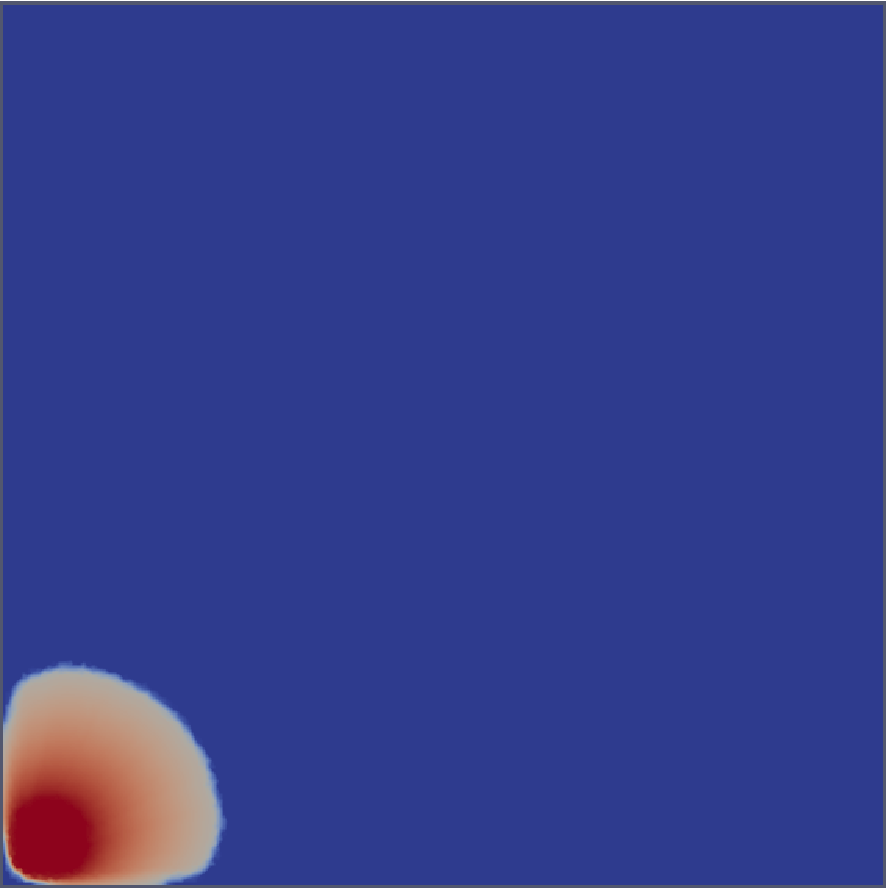
\includegraphics[width=.6\textwidth]{./Pics1/Saffman_homogeneous/saffman_homo_fixed_250_1.pdf}
}
\vspace{0.0cm}
\hbox{\hspace{5.0cm} (b) flow at t=250  
}
}     
\caption{This is a description of a Hele-Shaw experimental domain, when MR=$10$ showing the source and sink term as this is implied in this test-case followed by a screenshot of the flow at time, t=250(b). Screenshot will follow that describe the progression of the flow in figure \ref{fig:2b_homoheleshaw_10} and figure \ref{fig:2c_homoheleshaw_10}.}
\label{fig:2a_homoheleshaw_10}
\end{figure}
\clearpage

%%%%
%%%%  FIGURE
%%%%
\begin{figure}[ht] 
\vbox{
\hbox{\hspace{2.5cm}
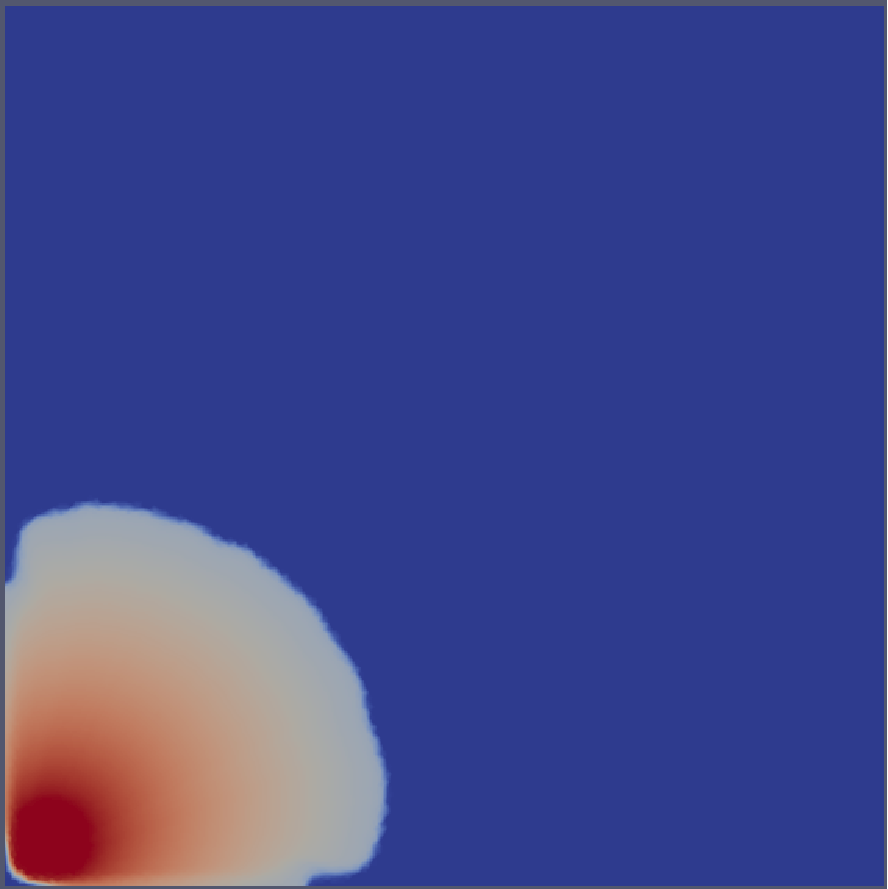
\includegraphics[width=.6\textwidth]{./Pics1/Saffman_homogeneous/saffman_homo_fixed_1000.pdf} 
}
\vspace{0.0cm}
\hbox{\hspace{5.0cm} (a) flow at t=1000   
}
\vspace{0.25cm}
\hbox{\hspace{2.5cm}
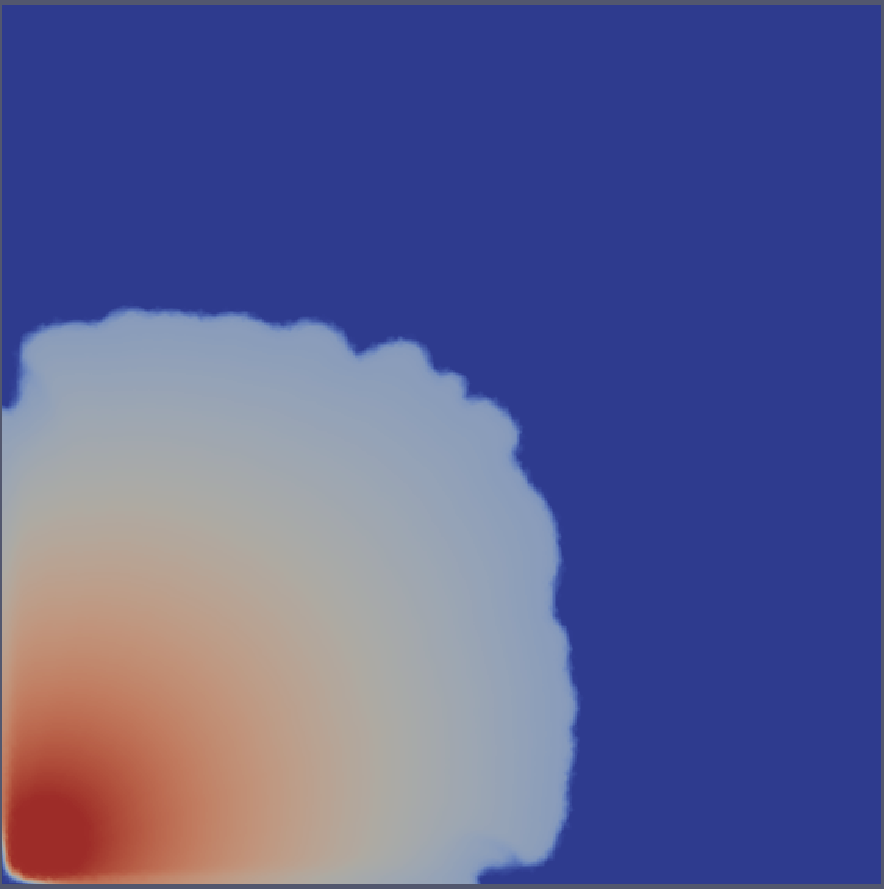
\includegraphics[width=.6\textwidth]{./Pics1/Saffman_homogeneous/saffman_homo_fixed_4000.pdf}
}
\vspace{0.0cm}
\hbox{\hspace{5.0cm} (b) flow at t=4000  
}
}     
\caption{As the flow progress at t=1000(a) the front still remains uniform. The first break down of the front is happening at t=4000(b) where $3$ tips start to come out of the main flow.}
\label{fig:2b_homoheleshaw_10}
\end{figure}
\clearpage

%%%%
%%%%  FIGURE
%%%%
\begin{figure}[ht]
\vbox{
\hbox{\hspace{2.5cm}
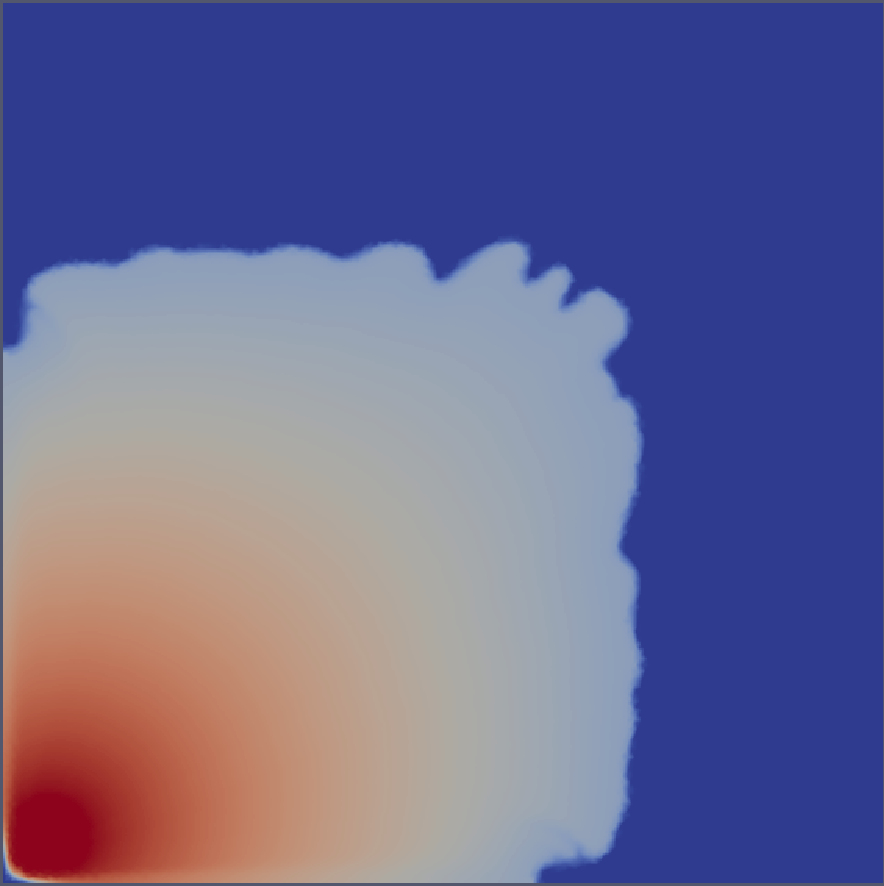
\includegraphics[width=.6\textwidth]{./Pics1/Saffman_homogeneous/saffman_homo_fixed_6000.pdf} 
}
\vspace{0.0cm}
\hbox{\hspace{5.0cm} (a) flow at t=6000   
}
\vspace{0.25cm}
\hbox{\hspace{2.5cm}
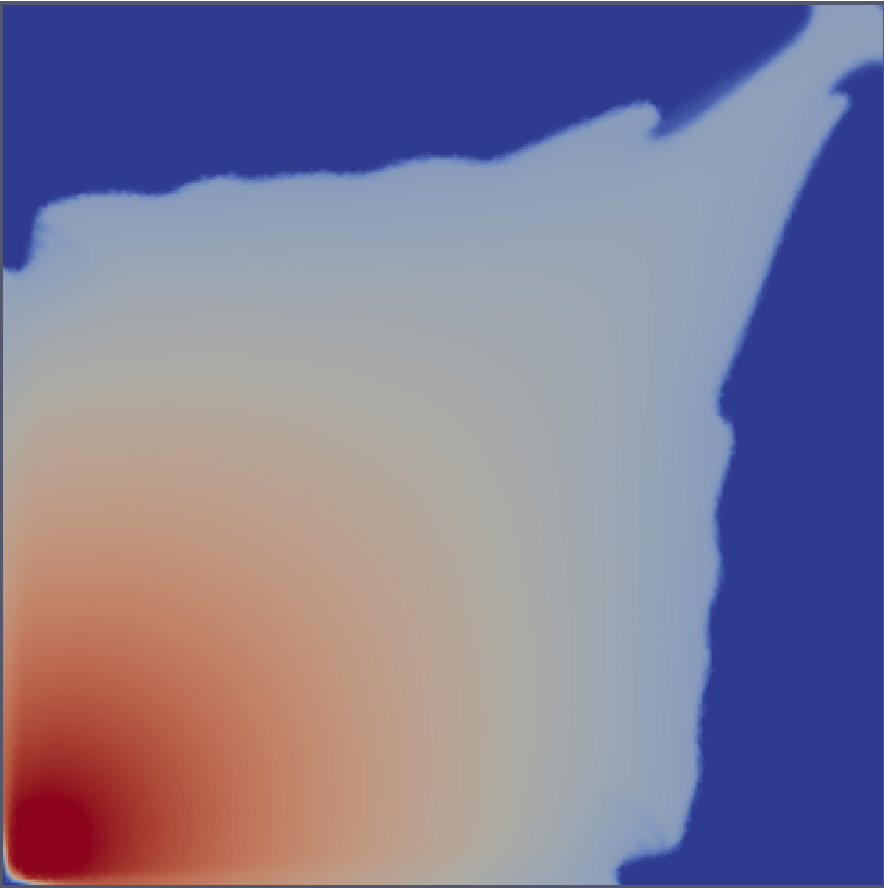
\includegraphics[width=.6\textwidth]{./Pics1/Saffman_homogeneous/saffman_homo_fixed_end_1.pdf}
}
\vspace{0.0cm}
\hbox{\hspace{5.0cm} (b) flow at t=end   
}
}     
\caption{Fingers are now more obvious as the flow progress and the tip-splitting mechanism becomes stronger at t=6000(a) as it approaches the area where sink term exist and finally at t=end(b) it will be absorbed.}
\label{fig:2c_homoheleshaw_10}
\end{figure}
\clearpage

%%%%
%%%%  FIGURE
%%%%
\begin{figure}[ht] 
\vbox{
\hbox{\hspace{2.5cm}
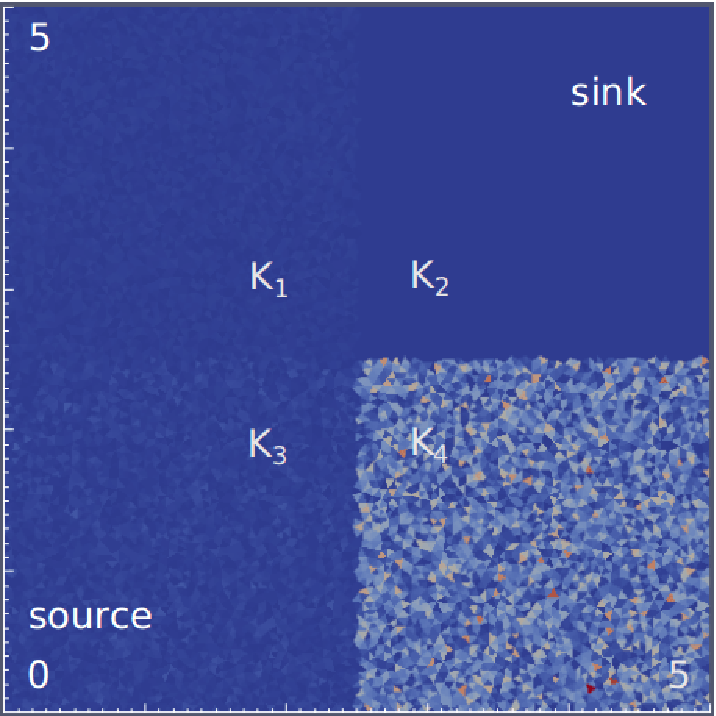
\includegraphics[width=.6\textwidth]{./Pics1/Saffman_heterogeneous/saffman_heter_fixed_1.pdf} 
}
\vspace{0.0cm}
\hbox{\hspace{4.5cm} (a) Hell-Shaw cell domain   
}
\vspace{0.25cm}
\hbox{\hspace{2.5cm}
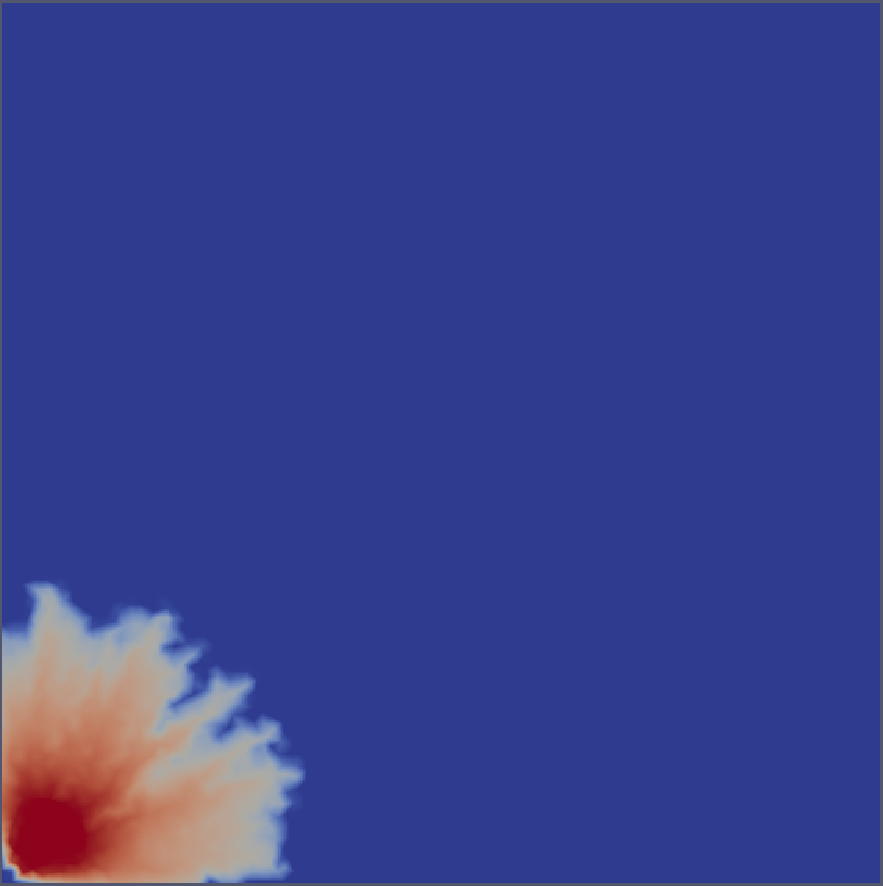
\includegraphics[width=.6\textwidth]{./Pics1/Saffman_heterogeneous/saffman_heter_fixed_500.pdf}
}
\vspace{0.0cm}
\hbox{\hspace{5.0cm} (b) flow at t=250     
}
}     
\caption{This is a description of a heterogeneous Hele-Shaw experimental domain, when MR=$10$ showing the source and sink term as this is implied in this test-case followed by a screenshot of the flow at time, t=500(b). Screenshot will follow that describe the progression of the flow in figure \ref{fig:3b_heteheleshaw_10} and figure \ref{fig:3c_heteheleshaw_10}.}
\label{fig:3a_heteheleshaw_10}
\end{figure}
\clearpage

%%%%
%%%%  FIGURE
%%%%
\begin{figure}[ht] 
\vbox{
\hbox{\hspace{2.5cm}
\includegraphics[width=.6\textwidth]{./Pics1/Saffman_heterogeneous/saffman_heter_fixed_2000.pdf} 
}
\vspace{0.0cm}
\hbox{\hspace{5.0cm} (a) flow at t=2000   
}
\vspace{0.25cm}
\hbox{\hspace{2.5cm}
\includegraphics[width=.6\textwidth]{./Pics1/Saffman_heterogeneous/saffman_heter_fixed_3000.pdf}
}
\vspace{0.0cm}
\hbox{\hspace{5.0cm} (b) flow at t=3000     
}
}     
\caption{As the flow progress at t=2000(a) but now the front is completely unstable as it has already collapsed forming many finger formations. Finger formations are more aggressive as the simulations progress, t=3000(b) where many tips have already start to develop out of the main flow.}
\label{fig:3b_heteheleshaw_10}
\end{figure}
\clearpage

%%%%
%%%%  FIGURE
%%%%
\begin{figure}[ht] 
\vbox{
\hbox{\hspace{2.5cm}
\includegraphics[width=.6\textwidth]{./Pics1/Saffman_heterogeneous/saffman_heter_fixed_6000.pdf} 
}
\vspace{0.0cm}
\hbox{\hspace{5.0cm} (a) flow at t=6000    
}
\vspace{0.25cm}
\hbox{\hspace{2.5cm}
\includegraphics[width=.6\textwidth]{./Pics1/Saffman_heterogeneous/saffman_heter_fixed_24000.pdf}
}
\vspace{0.0cm}
\hbox{\hspace{4.75cm} (b) flow at t=24000     
}
}     
\caption{At t=6000(a), one main finger have already reached the area where sink exists as they have develop much faster than the rest of the fingers. At t=24000(b) there are two main fingers that now have developed and drive the flow forwards.}
\label{fig:3c_heteheleshaw_10}
\end{figure}
\clearpage

%%%%
%%%%  FIGURE
%%%%
\begin{landscape}
\begin{figure}[ht] 
\vbox{
\hbox{\hspace{4.0cm}
\includegraphics[width=.8\textwidth]{./Pics/map_of_boundaries.pdf} 
}
\vspace{0.0cm}
\hbox{\hspace{6.5cm} (a) map of permeabilties K   
}
\vspace{0.25cm}
\hbox{\hspace{4.0cm}
\includegraphics[width=.8\textwidth]{./Pics/4r_po_adapt_fine_125_mesh.pdf}
}
\vspace{0.0cm}
\hbox{\hspace{9cm} (b)      
}
}     
\caption{(a) describes the initial and boundary conditions as these are applied in this set of simulations. Below (b) the unstructured and fixed mesh can been seen and there is a colored representation of permeabilities.}
\label{fig:testcase_heter_domain}
\end{figure}
\end{landscape}
\clearpage


%%%%
%%%%  FIGURE
%%%%
\begin{landscape}
\begin{figure}[ht] 
\vbox{
\hbox{\hspace{3.5cm}
\includegraphics[width=.8\textwidth]{./Pics1/mr10_5regions_fixed/5regions_fixed_250.pdf} 
}
\vspace{0.0cm}
\hbox{\hspace{6.5cm} (a) flow at t=250   
}
\vspace{0.25cm}
\hbox{\hspace{3.5cm}
\includegraphics[width=.8\textwidth]{./Pics1/mr10_5regions_adapt/5regions_adapt_250.pdf}
}
\vspace{0.0cm}
\hbox{\hspace{6.5cm} (b) flow at t=250     
}
}     
\caption{Start to compare $2$ test-cases under MR=$10$ and under fixed (top) and adaptive(bottom) mesh for t=250. There is a significant difference on the main front (left hand side of the domain) and the number of finger that appear.}
\label{fig:2testcase_a}
\end{figure}
\end{landscape}
\clearpage


%%%%
%%%%  FIGURE
%%%%
\begin{landscape}
\begin{figure}[ht] 
\vbox{
\hbox{\hspace{3.5cm}
\includegraphics[width=.8\textwidth]{./Pics1/mr10_5regions_fixed/5regions_fixed_500.pdf} 
}
\vspace{0.0cm}
\hbox{\hspace{6.5cm} (a) flow at t=500 (fixed mesh)   
}
\vspace{0.25cm}
\hbox{\hspace{3.5cm}
\includegraphics[width=.8\textwidth]{./Pics1/mr10_5regions_adapt/5regions_adapt_500.pdf}
}
\vspace{0.0cm}
\hbox{\hspace{6.5cm} (b) flow at t=500 (adaptive mesh)     
}
}     
\caption{Cross flow is taking place at the upper part of the formation. The fingers start to becoming more proufound for for the (b) case below.}
\label{fig:2testcase_b}
\end{figure}
\end{landscape}
\clearpage

%%%%
%%%%  FIGURE
%%%%
\begin{landscape}
\begin{figure}[ht] 
\vbox{
\hbox{\hspace{3.5cm}
\includegraphics[width=.8\textwidth]{./Pics1/mr10_5regions_fixed/5regions_fixed_1500.pdf} 
}
\vspace{0.0cm}
\hbox{\hspace{6.5cm} (a) flow at t=1500 (fixed mesh)   
}
\vspace{0.25cm}
\hbox{\hspace{3.5cm}
\includegraphics[width=.8\textwidth]{./Pics1/mr10_5regions_adapt/5regions_adapt_1500.pdf}
}
\vspace{0.0cm}
\hbox{\hspace{6.5cm} (b) flow at t=1500 (adaptive mesh)     
}
}     
\caption{Cross flow at the upper part has almost travel all the way towards the outlet (left-hand side) and the finger below start forming a front that is also travelling towards the left-hand side.}
\label{fig:2testcase_c}
\end{figure}
\end{landscape}
\clearpage

%%%%
%%%%  FIGURE
%%%%
\begin{landscape}
\begin{figure}[ht] 
\vbox{
\hbox{\hspace{3.5cm}
\includegraphics[width=.8\textwidth]{./Pics1/mr10_5regions_fixed/5regions_fixed_2000.pdf} 
}
\vspace{0.0cm}
\hbox{\hspace{6.5cm} (a) flow at t=end (fixed mesh)   
}
\vspace{0.25cm}
\hbox{\hspace{3.5cm}
\includegraphics[width=.8\textwidth]{./Pics1/mr10_5regions_adapt/5regions_adapt_3000.pdf}
}
\vspace{0.0cm}
\hbox{\hspace{6.5cm} (b) flow at t=end (adaptive mesh)     
}
}     
\caption{Using the $P_{1}DGP_{2}$ element type for MR=$10$ under the same time steps, we compared the impact of fixed and adaptive mesh. When adaptive mesh is introduce there is better repersentation of the fluid instabilities as these are developed on time.}
\label{fig:2testcase_d}
\end{figure}
\end{landscape}
\clearpage

%%%%
%%%%  FIGURE
%%%%
\begin{landscape}
\begin{figure}[ht] 
\vbox{
\hbox{\hspace{3.5cm}
\includegraphics[width=.8\textwidth]{./Pics1/mr10_5regions_fixed_dinlet/5regions_dinlet_fixed_100}
}
\vspace{0.0cm}
\hbox{\hspace{6.5cm} (a) double inlet - fixed mesh   
}
\hbox{\hspace{3.5cm}
  \includegraphics[width=.8\textwidth]{./Pics1/mr10_5regions_adapt_dinlet/5regions_dinlet_adapt_start}
}
\vspace{0.0cm}
\hbox{\hspace{6.5cm} (b) double inlet adaptive mesh   
}
}     
\caption{Comparing test-cases of fixed and adaptive mesh while we have a dual inlet, using the $P_{1}DGP_{2}$ element type for MR=$10$ under the same time steps}
\label{fig:3testcase_a}
\end{figure}
\end{landscape}
\clearpage

%%%%
%%%%  FIGURE
%%%%
\begin{figure}[ht] 
\vbox{
\hbox{\hspace{3.5cm}
\includegraphics[width=.5\textwidth]{./Pics1/mr10_5regions_adapt/5regions_adapt_vel_magn.pdf} 
}
\vspace{0.0cm}
\hbox{\hspace{5.0cm} (a) single inlet velocity magnitude   
}
\hbox{\hspace{3.5cm}
\includegraphics[width=.5\textwidth]{./Pics1/mr10_5regions_adapt_dinlet/5regions_dinlet_adapt_vel_magn.pdf}
}
\vspace{0.0cm}
\hbox{\hspace{5.0cm} (b) double inlet velocity magnitude   
}
}     
\caption{For the same time step, t=1000, these plots describe the velocity magnitudes of the phase $1$ (injected fluid) under the same boundary and initiall conditions. From top to bottom,these graphs describe the velocity magnitude %for fixed mesh is plotted(top), the velocity magnitude 
for adaptive mesh-single inlet (top) and the velocity magnitude for adaptive mesh with double inlet (bottom) as these are also presented in fig.\ref{fig:3testcase_a}. The main difference between the upper and lower plot %is not just the ability to capture in greater detail, the fluid instabilities as they happenduring the finger development and their velocity patterns. While there 
is the impact of the second injection interval as this can be seen from the slope and the rate that the velocity magnitude is changing.}
\label{fig:vel_magn}
\end{figure}

%%%%
%%%%  FIGURE
%%%%
\begin{landscape}
\begin{figure}[ht] 
\vbox{
\hbox{\hspace{3.5cm}
\includegraphics[width=.8\textwidth]{./Pics1/5reg_dinlet_fixed_500.pdf} 
}
\vspace{0.0cm}
\hbox{\hspace{6.5cm} (a) double inlet - fixed mesh   
}
\hbox{\hspace{3.5cm}
\includegraphics[width=.8\textwidth]{./Pics1/5reg_dinlet_adapt_500.pdf}
}
\vspace{0.0cm}
\hbox{\hspace{6.5cm} (b) double inlet adaptive mesh   
}
}     
\caption{for t=$500$ there is a comparison between fixed mesh(a) and adaptive mesh(b).}
\label{fig:3testcase_b}
\end{figure}
\end{landscape}
\clearpage

%%%%
%%%%  FIGURE
%%%%
\begin{landscape}
\begin{figure}[ht] 
\vbox{
\hbox{\hspace{3.5cm}
\includegraphics[width=.8\textwidth]{./Pics1/5reg_dinlet_fixed_1500.pdf} 
}
\vspace{0.0cm}
\hbox{\hspace{6.5cm} (a) double inlet - fixed mesh   
}
\hbox{\hspace{3.5cm}
\includegraphics[width=.8\textwidth]{./Pics1/5reg_dinlet_adapt_1500.pdf}
}
\vspace{0.0cm}
\hbox{\hspace{6.5cm} (b) double inlet adaptive mesh   
}
}     
\caption{for t=$1500$ there is a comparison between fixed mesh(a) and adaptive mesh(b).}
\label{fig:3testcase_c}
\end{figure}
\end{landscape}
\clearpage

%%%%
%%%%  FIGURE
%%%%
\begin{landscape}
\begin{figure}[ht] 
\vbox{
\hbox{\hspace{3.5cm}
\includegraphics[width=.8\textwidth]{./Pics1/5reg_dinlet_fixed_end.pdf} 
}
\vspace{0.0cm}
\hbox{\hspace{6.5cm} (a) double inlet - fixed mesh   
}
\hbox{\hspace{3.5cm}
\includegraphics[width=.8\textwidth]{./Pics1/5reg_dinlet_adapt_end.pdf}
}
\vspace{0.0cm}
\hbox{\hspace{6.5cm} (b) double inlet adaptive mesh   
}
}     
\caption{for t=$1500$ there is a comparison between fixed mesh(a) and adaptive mesh(b).}
\label{fig:3testcase_d}
\end{figure}
\end{landscape}
\clearpage

%%%%
%%%%  FIGURE
%%%%
\begin{landscape}
\begin{figure}[ht] 
\vbox{
\hbox{\hspace{3.5cm}
\includegraphics[width=.8\textwidth]{./Pics1/mr100_fixed/mr100_fixed_500.pdf} 
}
\vspace{0.0cm}
\hbox{\hspace{4.0cm} (a) fixed and unstructured mesh for MR = 100 (start)   
}
\hbox{\hspace{3.5cm}
\includegraphics[width=.8\textwidth]{./Pics1/mr100_fixed/mr100_fixed_1500.pdf}
}
\vspace{0.0cm}
\hbox{\hspace{3.75cm} (b) fixed and unstructured mesh for MR = 100 (t = 1500)   
}
}     
\caption{for the case of MR=$100$ from top to bottom, these are screenshots taken from the test-case of MR=$100$ using fixed and unstructured mesh for the same time steps, t=500(a), t=1500(b), t=3000(c), t=end(d) }
\label{fig:4testcase_a}
\end{figure}
\end{landscape}
\clearpage

%%%%
%%%%  FIGURE
%%%%
\begin{landscape}
\begin{figure}[ht] 
\vbox{
\hbox{\hspace{3.5cm}
\includegraphics[width=.8\textwidth]{./Pics1/mr100_fixed/mr100_fixed_3000.pdf} 
}
\vspace{0.0cm}
\hbox{\hspace{3.75cm} (a) fixed and unstructured mesh for MR = 100 (t = 3000)   
}
\hbox{\hspace{3.5cm}
\includegraphics[width=.8\textwidth]{./Pics1/mr100_fixed/mr100_fixed_end.pdf}
}
\vspace{0.0cm}
\hbox{\hspace{3.75cm} (b) fixed and unstructured mesh for MR = 100 (t = end)   
}
}     
\caption{for the case of MR=$100$ from top to bottom, these are screenshots taken from the test-case of MR=$100$ using fixed and unstructured mesh for the same time steps, t=3000(a), t=end(b) }
\label{fig:4testcase_b}
\end{figure}
\end{landscape}
\clearpage


